%%%%%%%%%%%%%%%%%%%%%%%%%%%%%%%%%%%%%%%%%%%%%%%%%%%%%%%%%%%%%%%%%%
%%%%%%%%%%%%%%%%%%%%%%%%%%%%%%%%%%%%%%%%%%%%%%%%%%%%%%%%%%%%%%%%%%
%\pagestyle{myheadings} \markright{Daniel Wollschläger \hfill Grundlagen der Datenanalyse mit R}
\chapter{Resampling-Verfahren}
\label{sec:resampling}
%%%%%%%%%%%%%%%%%%%%%%%%%%%%%%%%%%%%%%%%%%%%%%%%%%%%%%%%%%%%%%%%%%
%%%%%%%%%%%%%%%%%%%%%%%%%%%%%%%%%%%%%%%%%%%%%%%%%%%%%%%%%%%%%%%%%%

\index{Resampling-Verfahren}
Resampling-Verfahren kommen für eine Vielzahl von Tests in Frage, können hier aber nur in Grundzügen vorgestellt werden. Ausgangspunkt ist die gesuchte Verteilung einer Teststatistik $\hat{\theta}$ -- etwa eines Schätzers $\hat{\theta}$ für einen theoretischen Parameter $\theta$. Diese Verteilung kann aus verschiedenen Gründen unbekannt sein: So sind etwa die in parametrischen Tests gemachten Annahmen, unter denen ihre Teststatistik eine bekannte Verteilung aufweist, nicht immer zu rechtfertigen. In vielen klassischen nonparametrischen Verfahren ist die Verteilung der Teststatistik zwar im Prinzip exakt zu ermitteln, praktisch aber der Rechenaufwand dafür zu hoch.

Grundidee von Bootstrap-Verfahren und Permutationstests ist es, aus den gegebenen Daten einer festen Basisstichprobe viele neue Zufallsstichproben (\emph{resamples}) zu generieren und die Teststatistik für jedes resample zu ermitteln -- die dabei berechneten Werte werden als $\hat{\theta}^{\star}$ bezeichnet. Die empirische Verteilung der $\hat{\theta}^{\star}$ dient der Approximation der theoretischen Verteilung von $\hat{\theta}$. Die Beziehung zwischen resample und Basisstichprobe wird also auf die Beziehung zwischen Basisstichprobe und Population übertragen. Im Vergleich zu klassischen nonparametrischen Tests (Kap.\ \ref{sec:bioStat}) versprechen Resampling-Methoden oft eine höhere Power.

%%%%%%%%%%%%%%%%%%%%%%%%%%%%%%%%%%%%%%%%%%%%%%%%%%%%%%%%%%%%%%%%%%
%%%%%%%%%%%%%%%%%%%%%%%%%%%%%%%%%%%%%%%%%%%%%%%%%%%%%%%%%%%%%%%%%%
\section{Nonparametrisches Bootstrapping}
\label{sec:boot}
%%%%%%%%%%%%%%%%%%%%%%%%%%%%%%%%%%%%%%%%%%%%%%%%%%%%%%%%%%%%%%%%%%
%%%%%%%%%%%%%%%%%%%%%%%%%%%%%%%%%%%%%%%%%%%%%%%%%%%%%%%%%%%%%%%%%%

\index{Resampling-Verfahren!Bootstraping!Nonparametrisch}
\index{Bootstrap-Verfahren|see{Resampling-Verfahren}}
Bei Bootstrap-Verfahren \cite{Chihara2011,Davison1997} werden die resamples als \emph{Replikationen} bezeichnet. Beim nonparametrischen bootstrap sind dies mit Zurücklegen gezogene Zufallsstichproben aus der Basisstichprobe mit derem Stichprobenumfang. $\hat{\theta}$ ist der auf Grundlage der Basisstichprobe berechnete \emph{plug-in}-Schätzer von $\theta$, wird also auf empirischer Ebene rechnerisch genauso gebildet wie $\theta$ auf theoretischer Ebene.\footnote{$\theta$ ist ein \emph{Funktional} der theoretischen Verteilungsfunktion $F$ der ursprünglichen Zufallsvariable, bildet also $F$ auf eine Zahl ab. Analog ist $\hat{\theta}$ dasselbe Funktional der empirischen kumulativen Häufigkeitsverteilung $\hat{F}_{n}$ der Basisstichprobe vom Umfang $n$ und $\hat{\theta}^{\star}$ dasselbe Funktional der empirischen kumulativen Häufigkeitsverteilung $\hat{F}_{n}^{\star}$ in einer Replikation.} Über den -- oft weniger interessanten -- Bootstrap-Punktschätzer für $\theta$ hinaus lassen sich aus der empirischen Verteilung von $\hat{\theta}^{\star}$ vor allem Konfidenzintervalle für $\theta$ bestimmen. Dafür approximiert die empirische Verteilung von $\hat{\theta}^{\star} - \hat{\theta}$ in vielen Fällen jene der Pivot-Statistik $\hat{\theta} - \theta$, deren Verteilung unabhängig vom konkreten Wert für $\theta$ ist.

Ein vollständiger nonparametrischer bootstrap umfasst alle möglichen Replikationen einer Basisstichprobe vom Umfang $n$, wofür der Rechenaufwand jedoch meist zu groß ist: Es gibt bereits $2^{n} - 1$ relevante Teilmengen von Beobachtungsobjekten (die Mächtigkeit der Potenzmenge ohne die leere Menge), wobei die Elemente jeder denkbaren Zusammensetzung noch mit unterschiedlichen Häufigkeiten berücksichtigt werden können. Deswegen wird bootstrapping als \emph{Monte-Carlo-Verfahren} durchgeführt und nur eine zufällige Auswahl von Replikationen berücksichtigt.

%%%%%%%%%%%%%%%%%%%%%%%%%%%%%%%%%%%%%%%%%%%%%%%%%%%%%%%%%%%%%%%%%%
%%%%%%%%%%%%%%%%%%%%%%%%%%%%%%%%%%%%%%%%%%%%%%%%%%%%%%%%%%%%%%%%%%
\subsection{Replikationen erstellen}
\label{sec:bootFun}
%%%%%%%%%%%%%%%%%%%%%%%%%%%%%%%%%%%%%%%%%%%%%%%%%%%%%%%%%%%%%%%%%%
%%%%%%%%%%%%%%%%%%%%%%%%%%%%%%%%%%%%%%%%%%%%%%%%%%%%%%%%%%%%%%%%%%

Das Paket\index[pack]{boot@\lstinline{boot}} \lstinline!boot! stellt mit\index[func]{boot()@\lstinline{boot()}} \lstinline!boot()! eine Funktion bereit, die Bootstrap-Replikationen durchführt.
\begin{lstlisting}
boot(data=<<Basisstichprobe>>, statistic=<<Funktion>>,
     R=<<Anzahl Replikationen>>, strata=<<Faktor>>)
\end{lstlisting}

Für \lstinline!data! ist der Vektor mit den Werten der Basisstichprobe zu übergeben. Basiert $\hat{\theta}$ auf Daten mehrerer Variablen, muss \lstinline!data! ein Datensatz mit diesen Variablen sein. Das Argument \lstinline!statistic! erwartet den Namen einer Funktion mit ihrerseits zwei Argumenten zur Berechnung von $\hat{\theta}^{\star}$: Ihr erstes Argument ist ebenfalls der Vektor bzw.\ Datensatz der Basisstichprobe. Das zweite Argument der für \lstinline!statistic! genannten Funktion ist ein numerischer Indexvektor, dessen Elemente sich auf die Beobachtungsobjekte beziehen. \lstinline!boot()! ruft für jede der \lstinline!R! vielen Replikationen \lstinline!statistic! auf und übergibt die Basis-Daten samt eines zufällig gewählten Indexvektors als Anweisung, wie eine konkrete Replikation aus Fällen der Basisstichprobe zusammengesetzt sein soll.

Das Ergebnis der für \lstinline!statistic! genannten Funktion muss $\hat{\theta}^{\star}$ sein -- sind gleichzeitig mehrere Parameter $\theta_{j}$ zu schätzen, analog ein Vektor mit den $\hat{\theta}^{\star}_{j}$. Um beim bootstrapping eine vorgegebene Stratifizierung der Stichprobe beizubehalten, kann ein Faktor an \lstinline!strata! übergeben werden, der eine Gruppeneinteilung definiert. In den Replikationen sind die Gruppengrößen dann gleich jenen der Basisstichprobe.

Als Beispiel diene die Situation eines $t$-Tests für eine Stichprobe auf einen festen Erwartungswert $\mu_{0}$ (Abschn.\ \ref{sec:tOne}). Ziel im folgenden Abschnitt ist die Konstruktion eines Vertrauensintervalls für $\mu$ ($= \theta_{1}$). Die Stichprobengröße sei $n$, der Mittelwert $M$ ($= \hat{\theta}_{1}$) und die unkorrigierte Varianz des Mittelwertes $S_{M}^{2}$ ($= \hat{\sigma}_{\hat{\theta_{1}}}^{2} = \hat{\theta}_{2}$) als plug-in-Schätzer der theoretischen Varianz $\sigma_{M}^{2}$ ($= \theta_{2}$). Dazu ist aus jeder Bootstrap-Replikation der Mittelwert $M^{\star}$ ($= \hat{\theta}_{1}^{\star}$) und die unkorrigierte Varianz des Mittelwertes $S_{M}^{2 \star}$ ($= \hat{\sigma}_{\hat{\theta_{1}}}^{2 \star} = \hat{\theta}_{2}^{\star}$) zu berechnen. Für das Erstellen eigener Funktionen s.\ Abschn.\ \ref{sec:function}.
\begin{lstlisting}
> muH0 <- 100                               # Erwartungswert unter H0
> sdH0 <- 40                                # Streuung unter H0
> N    <- 200                               # Größe Basisstichprobe
> DV   <- rnorm(N, muH0, sdH0)              # Basisstichprobe

# Mittelwert M* & Varianz des Mittelwertes S(M)^2* aus BS-Replikation,
# deren zufällige Zusammensetzung durch Indexvektor idx bestimmt wird
> getM <- function(orgDV, idx) {
+     n     <- length(orgDV[idx])
+     bsM   <- mean(orgDV[idx])                       # M*
+     bsS2M <- (((n-1)/n) * var(orgDV[idx])) / n      # S(M)^2*
+     c(bsM, bsS2M)
}

> library(boot)                             # für boot(), boot.ci()
> nR     <- 999                             # Anzahl BS-Replikationen
> (bsRes <- boot(DV, statistic=getM, R=nR)) # Bootstrap-Replikationen
ORDINARY NONPARAMETRIC BOOTSTRAP            # Ausgabe gekürzt ...
Bootstrap Statistics :
       original          bias   std. error
t1*  102.655867   -0.09535249     3.057508
t2*    9.162478   -0.02025724     0.881103
\end{lstlisting}

Die Ausgabe von \lstinline!boot()! nennt in den Zeilen \lstinline!t1*! und \lstinline!t2*! Eigenschaften der von \lstinline!statistic! zurückgegebenen Bootstrap-Schätzer: In der Spalte \lstinline!original! stehen die für die Basisstichprobe berechneten Werte. Hier sind dies der Mittelwert und seine unkorrigierte Varianz. In der Spalte \lstinline!bias! folgt die Verzerrung jedes Bootstrap-Schätzers als Mittelwert der Abweichungen $\hat{\theta}^{\star} - \hat{\theta}$. Für die Punktschätzung von $\theta$ kann sie zu einer einfachen Bias-Korrektur eingesetzt werden, indem sie von $\hat{\theta}$ abgezogen wird. Schließlich folgt in der Spalte \lstinline!std. error! die korrigierte Streuung für jeden Kennwert der pro Replikation von \lstinline!statistic! berechneten Kennwerte. Diese sind in der von \lstinline!boot()! zurückgegebenen Liste spaltenweise als Matrix in der Komponente \lstinline!t! gespeichert.
\begin{lstlisting}
> (M <- mean(DV))                         # Mittelwert Basisstichprobe
[1] 102.6559

> (S2M <- (((N-1)/N) * var(DV)) / N)      # unkorrigierte Varianz von M
[1] 9.162478

> Mstar   <- bsRes$t[ , 1]                # M* jeder Replikation
> S2Mstar <- bsRes$t[ , 2]                # S(M)^2* jeder Replikation
> (biasM  <- mean(Mstar) - M)             # Bias-Schätzung für M
[1] -0.0953525

> mean(S2Mstar) - S2M                     # Bias-Schätzung für S(M)^2
[1] -0.02025724

> c(sd(Mstar), sd(S2Mstar))               # Streuungen der BS-Kennwerte
[1] 3.057508 0.881103
\end{lstlisting}

Die Verteilung von $\hat{\theta}^{\star} - \hat{\theta}$ sollte unimodal und symmetrisch sein, nicht unähnlich einer Normalverteilung (Abb.\ \ref{fig:bootHist}). Dies lässt sich etwa durch ein Histogramm mit eingezeichneter Dichtefunktion einer passenden Normalverteilung zusammen mit einem nonparametrischen Kerndichteschätzer oder einem Q-Q-Plot prüfen.
\begin{lstlisting}
> hist(Mstar-M, freq=FALSE, breaks="FD")  # Histogramm von M* - M
> rug(jitter(Mstar-M))                    # Einzelwerte der M* - M

# Dichtefunktion einer Normalverteilung
> curve(dnorm(x, mean(Mstar-M), sd(Mstar-M)),
+       lwd=2, col="blue", add=TRUE)

> lines(density(Mstar-M), lwd=2, col="red", lty=2) # Kerndichteschätzer
> qqnorm(Mstar-M, pch=16)                 # Q-Q-Plot der M* - M
> qqline(Mstar-M, lwd=2, col="blue")      # Normalverteilung-Referenz
\end{lstlisting}

\begin{figure}[ht]
\centering
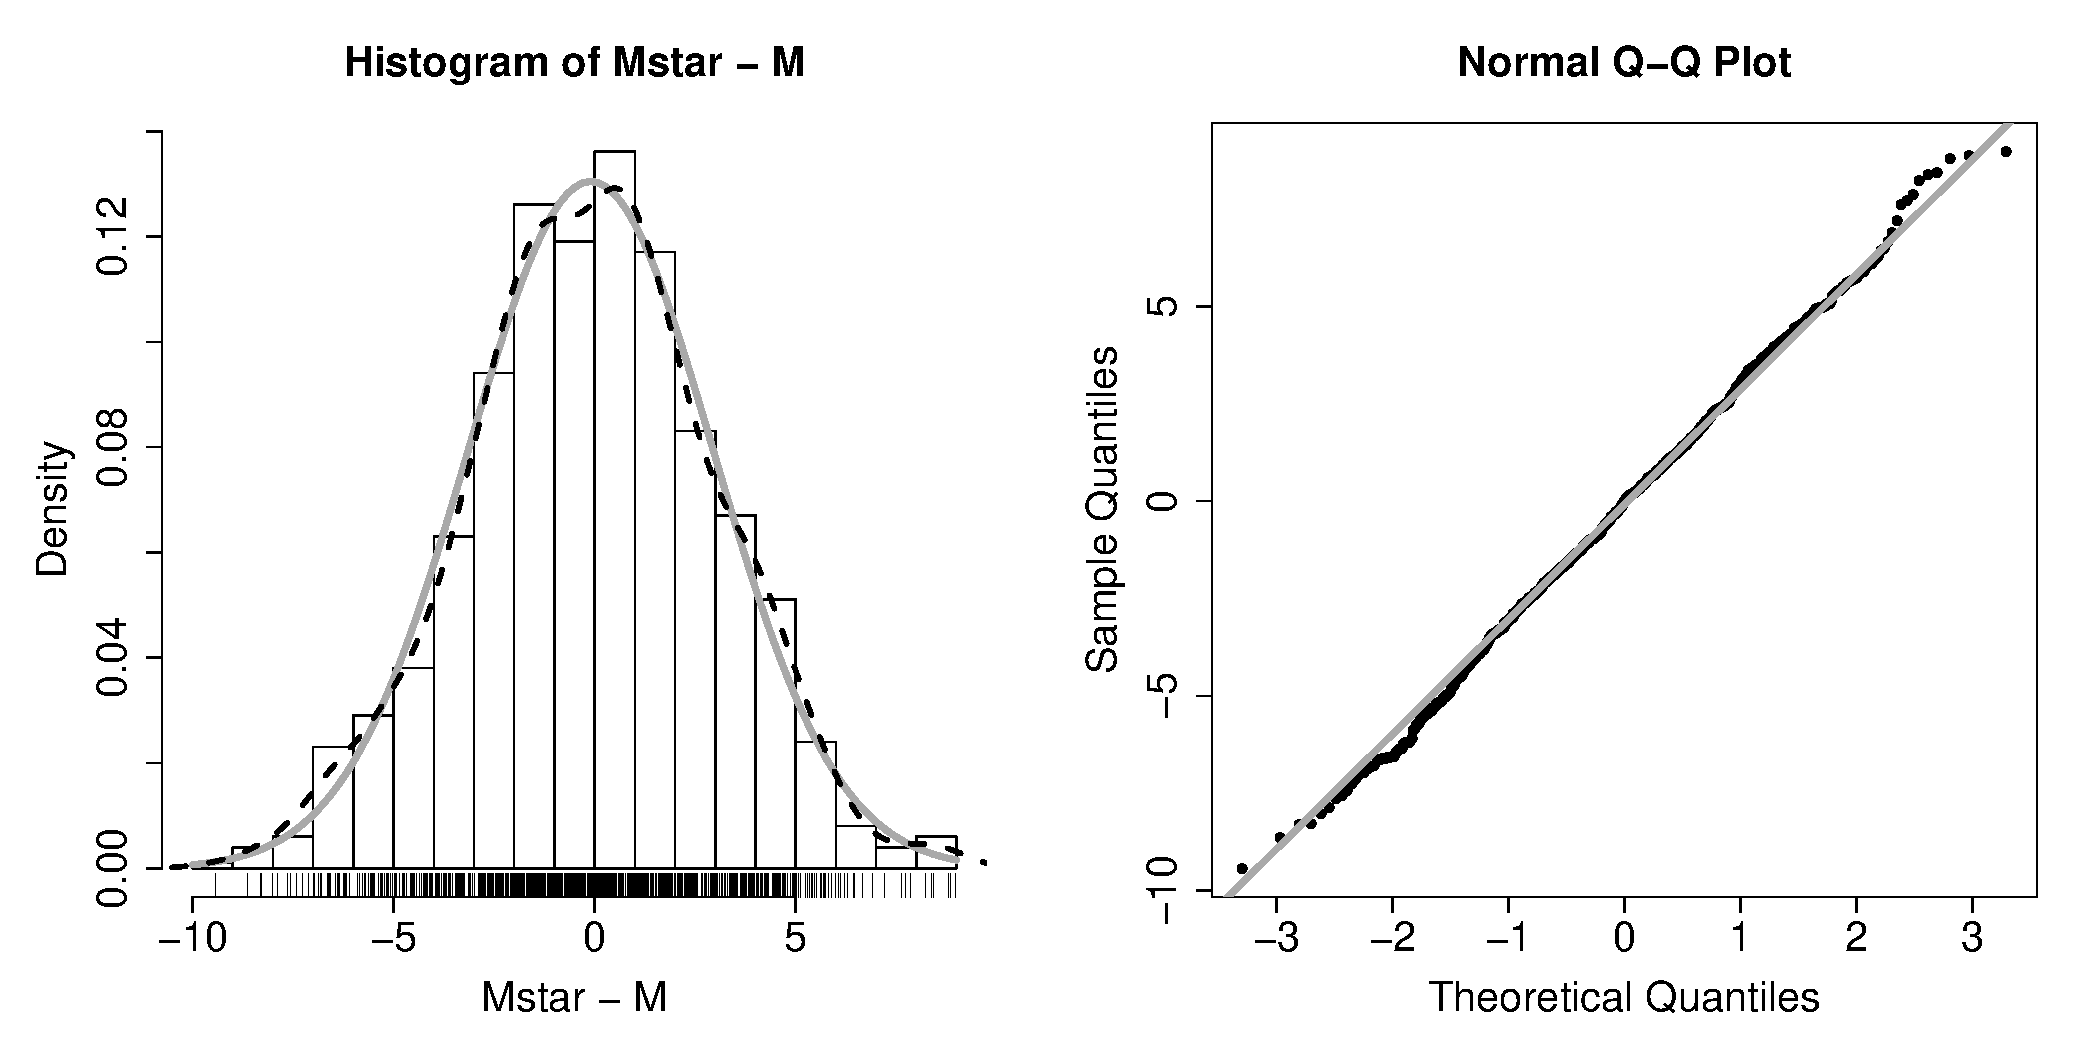
\includegraphics[width=12.5cm]{bootHist}
\vspace*{-0.5em}
\caption{Histogramm von $M^{\star}-M$ aus Bootstrap-Replikationen mit passender Normalverteilung und nonparametrischem Kerndichteschätzer. Q-Q-Plot von $M^{\star}-M$ mit Vergleich zur Standardnormalverteilung.}
\label{fig:bootHist}
\end{figure}

Detaillierte Informationen über die Zusammensetzung aller von \lstinline!boot()! erstellten Replikationen liefert\index[func]{booty.array()@\lstinline{boot.array()}} \lstinline!boot.array(<<boot-Objekt>>, indices=TRUE)!. Bei einer Basisstichprobe vom Umfang $n$ und $R$ Replikationen ist das Ergebnis mit dem Argument \lstinline!indices=TRUE! eine $(R \times  n)$-Matrix mit einer Zeile für jede Replikation und einer Spalte pro Beobachtung. Die Zelle $(r, i)$ enthält den Index des ausgewählten Elements der Basisstichprobe. Zusammen mit dem Vektor der Basisstichprobe lassen sich damit alle Replikation rekonstruieren.
\begin{lstlisting}
# Replikationen 1-3: je ausgewählte erste 10 Indizes Basisstichprobe
> bootIdx <- boot.array(bsRes, indices=TRUE)
> bootIdx[1:3, 1:10]
     [,1] [,2] [,3] [,4] [,5] [,6] [,7] [,8] [,9] [,10]
[1,]   78  148   83   72   86   78   33   59   87   141
[2,]   41  116  197   87  183    4  102  129   84   175
[3,]  123  107   60  181   35  133  196  197   15    71

> repl1Idx <- bootIdx[1, ]        # Indizes der ersten Replikation
> repl1DV  <- DV[repl1Idx]        # Werte der ersten Replikation
> head(repl1DV, n=5)
[1]  86.12395  72.41568 135.87073 149.96011  99.03936
\end{lstlisting}

%%%%%%%%%%%%%%%%%%%%%%%%%%%%%%%%%%%%%%%%%%%%%%%%%%%%%%%%%%%%%%%%%%
%%%%%%%%%%%%%%%%%%%%%%%%%%%%%%%%%%%%%%%%%%%%%%%%%%%%%%%%%%%%%%%%%%
\subsection[Bootstrap-Vertrauensintervalle für \texorpdfstring{$\mu$}{mu}]{Bootstrap-Vertrauensintervalle für \bm{$\mu$}}
\label{sec:bootMu}
%%%%%%%%%%%%%%%%%%%%%%%%%%%%%%%%%%%%%%%%%%%%%%%%%%%%%%%%%%%%%%%%%%
%%%%%%%%%%%%%%%%%%%%%%%%%%%%%%%%%%%%%%%%%%%%%%%%%%%%%%%%%%%%%%%%%%

\index{Resampling-Verfahren!Konfidenzintervalle}
\index[func]{boot.ci()@\lstinline{boot.ci()}}
Ein von \lstinline!boot()! erzeugtes Objekt ist für das Argument \lstinline!boot.out! der Funktion \lstinline!boot.ci()! anzugeben, die das zweiseitige Konfidenzintervall für $\theta$ bestimmt.
\begin{lstlisting}
boot.ci(boot.out=<<boot-Objekt>>, conf=<<Breite VI>>, index=<<Nummer>>,
        type="<<Methode>>")
\end{lstlisting}

Gibt die für \lstinline!boot(..., statistic)! genannte Funktion bei jedem Aufruf $J$ geschätzte Parameter zurück, ist \lstinline!index! der Reihe nach auf $1, \ldots, J$ zu setzen, um das zugehörige Konfidenzintervall zu erhalten. Das Intervall wird mit der Breite \lstinline!conf! nach einer über \lstinline!type! festzulegenden Methode gebildet:
\begin{itemize}
\item \lstinline!"basic"!: Das klassische Bootstrap-Intervall um $\hat{\theta}$, dessen Breite durch die $\frac{\alpha}{2}$- und $1-\frac{\alpha}{2}$-Quantile der Werte von $\hat{\theta} - \hat{\theta}^{\star}$ definiert ist.
\item \lstinline!"perc"!: Das Perzentil-Intervall, dessen Grenzen die $\frac{\alpha}{2}$- und $1-\frac{\alpha}{2}$-Quantile der Werte von $\hat{\theta}^{\star}$ sind.
\item \lstinline!"norm"!: Das Normalverteilungs-Intervall mit dem Zentrum in $\hat{\theta} - M(\hat{\theta}^{\star} - \hat{\theta})$ (Bias-Korrektur), dessen Breite definiert ist durch die $\frac{\alpha}{2}$- und $1-\frac{\alpha}{2}$-Quantile der Standardnormalverteilung multipliziert mit der Streuung von $\hat{\theta}^{\star}$.
\item \lstinline!"stud"!: Das $t$-Vertrauensintervall um $\hat{\theta}$, dessen Breite definiert ist durch die $\frac{\alpha}{2}$- und $1-\frac{\alpha}{2}$-Quantile der Werte von $t^{\star} = \frac{\hat{\theta}^{\star} - \hat{\theta}}{S_{\hat{\theta}}^{\star}}$ multipliziert mit der Streuung von $\hat{\theta}^{\star}$. Voraussetzung ist, das die Funktion \lstinline!statistic! als zweites Element den plug-in Schätzer $S_{\hat{\theta}}^{2 \star}$ der theoretischen Varianz $\sigma_{\hat{\theta}}^{2}$ zurückliefert. Ist deren geschlossene Form unbekannt oder existiert nicht, lässt sich $S_{\hat{\theta}}^{2 \star}$ innerhalb jedes Aufrufs von \lstinline!statistic! im ursprünglichen bootstrapping durch eine eigene (\emph{nested}) Bootstrap-Schätzung ermitteln.
\item \lstinline!"bca"!: Das $BC_{a}$-Intervall (\emph{bias-corrected and accelerated}). Für symmetrische Verteilungen und Schätzer mit geringem bias ähnelt es dem Perzentil- und $t$-Intervall meist stark. Bei schiefen Verteilungen und größerem bias wird das $BC_{a}$-Intervall den anderen oft vorgezogen.
\end{itemize}

Bei den Intervallen gehen zur Erhöhung der Genauigkeit nicht die $\frac{\alpha}{2}$- und $1-\frac{\alpha}{2}$-Quantile selbst von $t^{\star}$ bzw.\ von $\hat{\theta}^{\star}$ ein, die mit \lstinline!quantile(..., probs=c(<<alpha>>/2, 1 - <<alpha>>/2))! zu ermitteln wären: Bei $n_{R}$ vielen Replikationen sind dies stattdessen die Elemente mit den Indizes $(n_{R}+1) \cdot \frac{\alpha}{2}$ und $(n_{R}+1) \cdot (1-\frac{\alpha}{2})$ der sortierten Werte von $t^{\star}$ bzw. von $\hat{\theta}^{\star}$. Ergibt sich kein ganzzahliges Ergebnis für die Indizes, interpoliert \lstinline!boot.ci()! jeweils zwischen den angrenzenden Elementen.
\begin{lstlisting}
> alpha <- 0.05                            # alpha-Niveau
> boot.ci(bsRes, conf=1-alpha,
+         type=c("basic", "perc", "norm", "stud", "bca"))
BOOTSTRAP CONFIDENCE INTERVAL CALCULATIONS # gekürzte Ausgabe ...
Based on 999 bootstrap replicates
Intervals :
Level      Normal             Basic         Studentized
95%   ( 96.8, 108.7 )   ( 97.0, 109.1 )   ( 96.7, 109.0 )

Level     Percentile            BCa
95%   ( 96.2, 108.3 )   ( 96.2, 108.3 )
Calculations and Intervals on Original Scale
\end{lstlisting}

Es folgt die manuelle Kontrolle, zunächst für die Indizes $(n_{R}+1) \cdot \frac{\alpha}{2}$ und $(n_{R}+1) \cdot (1-\frac{\alpha}{2})$.
\begin{lstlisting}
> (idx <- trunc((nR + 1) * c(alpha/2, 1 - alpha/2)))
[1] 25 975

> tStar <- (Mstar-M) / sqrt(S2Mstar)       # t*
> tCrit <- sort(tStar)[idx]                # 2.5%, 97.5%-Quantil von t*
> zCrit <- qnorm(c(alpha/2, 1 - alpha/2))  # 2.5%, 97.5%-Quantil N(0,1)
> (ciBasic <- 2*M - sort(Mstar)[idx])      # klassisches VI
[1] 109.11192  96.97443

> (ciPerc <- sort(Mstar)[idx])             # Perzentil-VI
[1] 96.19981 108.33731

> (ciNorm <- M-biasM - zCrit*sd(Mstar))    # N(0, 1)-VI
[1] 108.74383  96.75861

> (ciT <- M - tCrit*sqrt(S2M))             # t-VI
[1] 108.99497  96.70034
\end{lstlisting}

Bei der manuellen Umsetzung der Bootstrap-Schätzungen sollen als Maß für deren Güte die kumulierten relativen Häufigkeiten von $t^{\star} = \frac{M^{\star}-M}{S_{M}^{\star}}$ mit der Verteilungsfunktion von $t = \frac{M - \mu_{0}}{s / \sqrt{n}}$ verglichen werden (mit $s$ als korrigierter Streuung). Im Fall $n$ unabhängiger Realisierungen einer normalverteilten Variable ist dies die $t_{n-1}$ Verteilung (Abb.\ \ref{fig:bootstrap}).
\begin{lstlisting}
# M*, S(M)* und t* aus Bootstrap-Replikationen
> res   <- replicate(nR, getM(DV, sample(seq(along=DV), replace=TRUE)))
> Mstar <- res[1, ]                        # M*
> SMstar <- sqrt(res[2, ])                 # S(M)*
> tStar  <- (Mstar-mean(DV)) / SMstar      # t*

# kumulierte relative Häufigkeiten von t*
> plot(tStar, ecdf(tStar)(tStar), col="gray60", pch=1,
+      xlab="t* bzw. t", ylab="P(T <= t)",
+      main="t*: Kumulierte relative Häufigkeiten")

# theoretische Verteilungsfunktion von t und Legende
> curve(pt(x, N-1), lwd=2, add=TRUE)
> legend(x="topleft", lty=c(NA, 1), pch=c(1, NA),
+        lwd=c(2, 2), col=c("gray60", "black"), legend=c("t*", "t"))
\end{lstlisting}

\begin{figure}[ht]
\centering
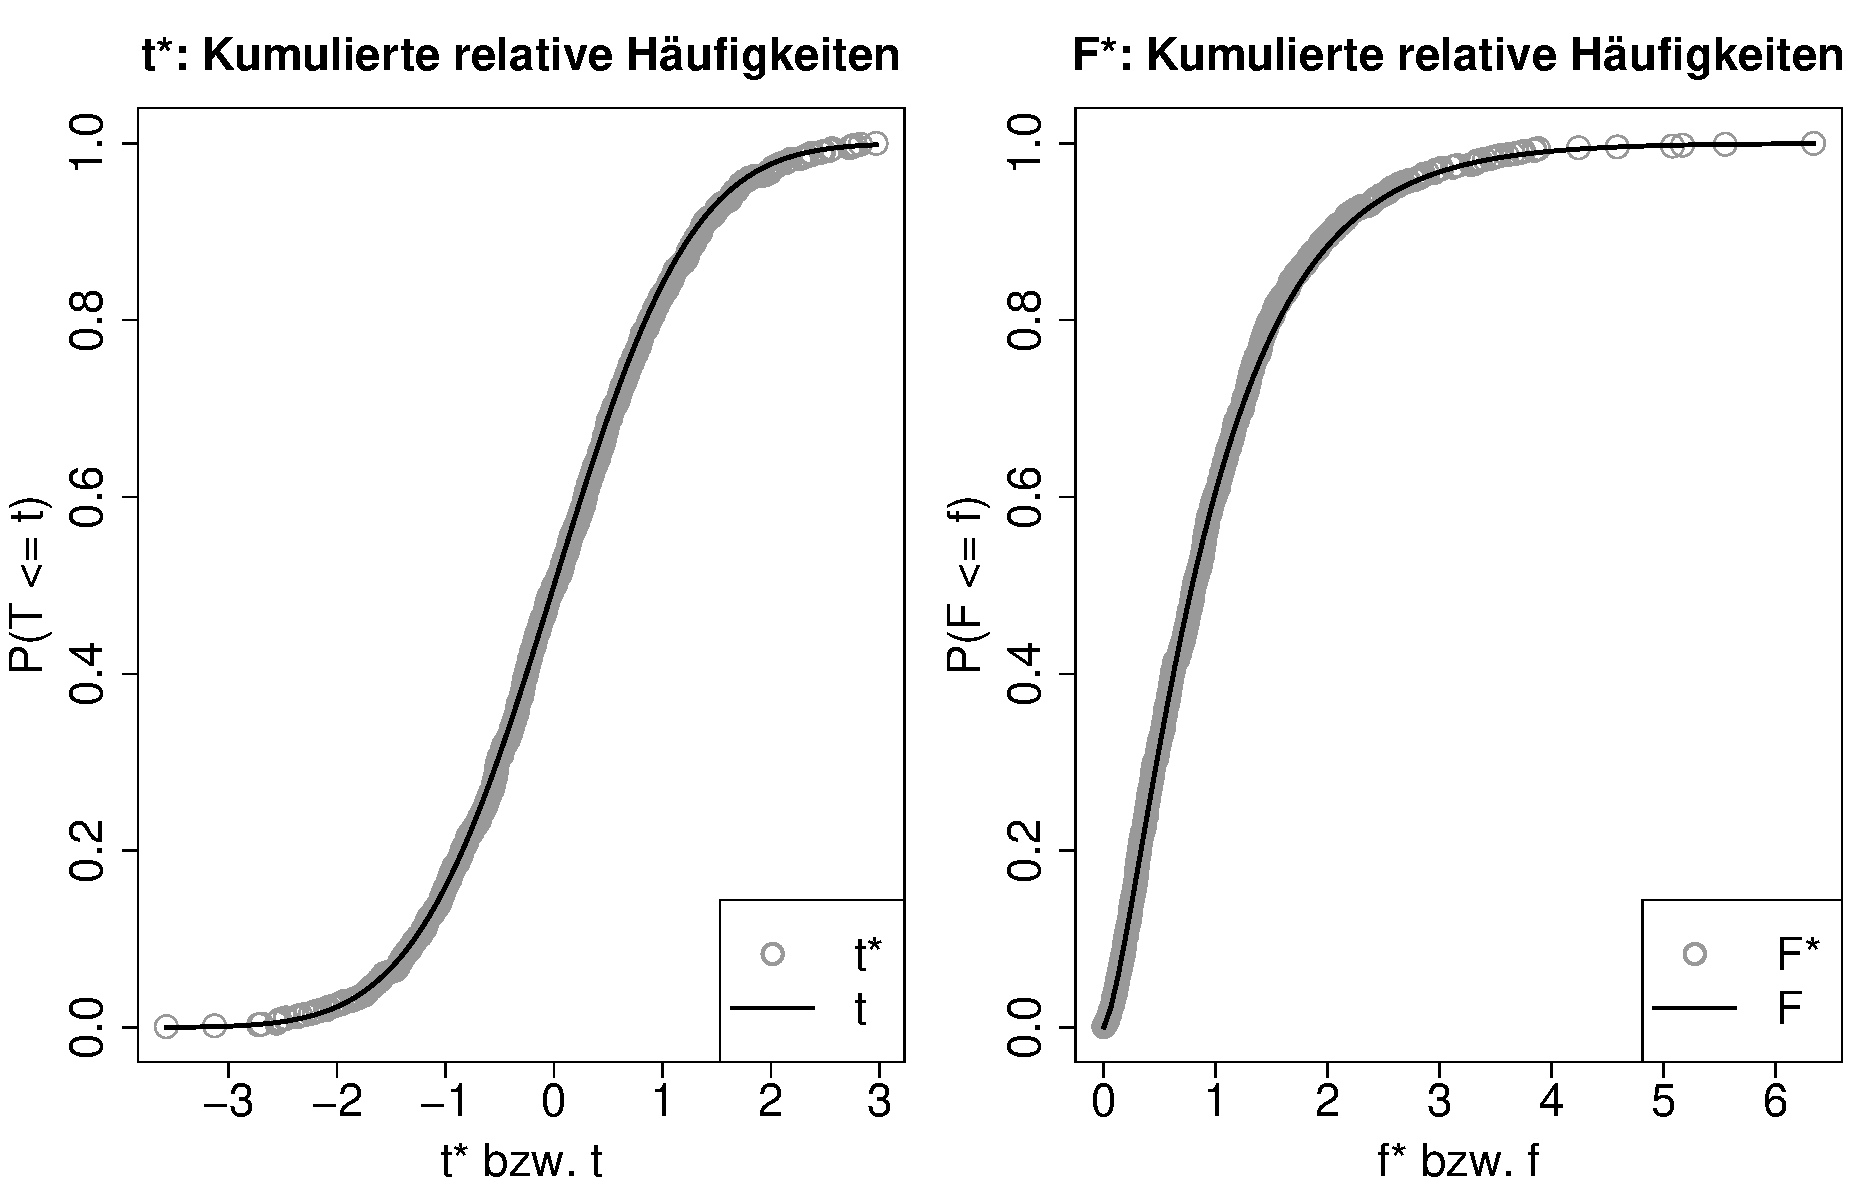
\includegraphics[width=12.5cm]{bootMuAnova}
\vspace*{-0.5em}
\caption{Kumulierte relative Häufigkeiten von $t^{\star}$ aus Bootstrap-Replikationen mit theoretischer Verteilungsfunktion $t_{n-1}$. Kumulierte relative Häufigkeiten von $F^{\star}$ aus Bootstrap-Replikationen mit theoretischer Verteilungsfunktion $F_{p-1,\, n-p}$.}
\label{fig:bootstrap}
\end{figure}

%%%%%%%%%%%%%%%%%%%%%%%%%%%%%%%%%%%%%%%%%%%%%%%%%%%%%%%%%%%%%%%%%%
%%%%%%%%%%%%%%%%%%%%%%%%%%%%%%%%%%%%%%%%%%%%%%%%%%%%%%%%%%%%%%%%%%
\subsection[Bootstrap-Vertrauensintervalle für \texorpdfstring{$\mu_{2}-\mu_{1}$}{mu2-mu1}]{Bootstrap-Vertrauensintervalle für \bm{$\mu_{2}-\mu_{1}$}}
\label{sec:bootTwoInd}
%%%%%%%%%%%%%%%%%%%%%%%%%%%%%%%%%%%%%%%%%%%%%%%%%%%%%%%%%%%%%%%%%%
%%%%%%%%%%%%%%%%%%%%%%%%%%%%%%%%%%%%%%%%%%%%%%%%%%%%%%%%%%%%%%%%%%

\index{Resampling-Verfahren!Bootstraping!Konfidenzintervalle}
\index{Resampling-Verfahren!Bootstraping!stratifiziert}
In der Situation eines $t$-Tests für zwei unabhängige Stichproben (Abschn.\ \ref{sec:tTwoInd}) kann bootstrapping eine nonparametrische Schätzung des Konfidenzintervalls für die Differenz der Erwartungswerte $\theta = \mu_{2}-\mu_{1}$ liefern. In der Basisstichprobe ist die Differenz der Gruppenmittelwerte $\hat{\theta} = M_{2}-M_{1}$ ein Schätzer für $\theta$, in jeder Replikation analog $\hat{\theta}^{\star} = M_{2}^{\star}-M_{1}^{\star}$. Für die Replikationen ist zu beachten, dass jeweils innerhalb jeder Gruppe mit Zurücklegen aus der Basisstichprobe gezogen wird, damit Gruppenzugehörigkeit und Gruppengrößen erhalten bleiben. Dies lässt sich mit dem Argument \lstinline!strata! von \lstinline!boot()! erreichen. Als Beispiel diene jenes aus Abschn.\ \ref{sec:tTwoInd} mit einer bei Frauen und Männern erhobenen Variable.
\begin{lstlisting}
# Datensatz aus Variable bei Männern, bei Frauen und Gruppierungsfaktor
> n1  <- 18                               # Stichprobenumfang 1
> n2  <- 21                               # Stichprobenumfang 2
> DVm <- rnorm(n1, 180, 10)               # Stichprobe Männer
> DVf <- rnorm(n2, 175, 6)                # Stichprobe Frauen
> tDf <- stack(list(m=DVm, f=DVf))        # Gesamt-Daten, erste Stufe m

# Funktion, um Differenz der Mittelwerte von f und m zu berechnen
> getDM <- function(dat, idx) {
+     # Gruppenmittelwerte für durch idx definierte Beobachtungen
+     Mfm <- aggregate(values ~ ind, data=dat, subset=idx, FUN=mean)
+     -diff(Mfm$values)  # M-Differenz, Reihenfolge m-f wie in t.test()
+ }

> library(boot)                             # für boot(), boot.ci()
> bsTind <- boot(tDf, statistic=getDM, strata=tDf$ind, R=999)
> boot.ci(bsTind, conf=0.95, type=c("basic", "bca"))
BOOTSTRAP CONFIDENCE INTERVAL CALCULATIONS  # gekürzte Ausgabe ...
Based on 999 bootstrap replicates
Intervals :
Level      Basic                BCa
95%   (-0.810,  7.709)   ( 0.096,  8.725)
Calculations and Intervals on Original Scale
\end{lstlisting}

Als Vergleich diene das parametrische Konfidenzintervall aus dem zugehörigen $t$-Test.
\begin{lstlisting}
> tt <- t.test(values ~ ind, alt="two.sided", var.equal=TRUE, data=tDf)
> tt$conf.int
[1] -0.8963473  8.3796152
\end{lstlisting}

Die analoge Situation mit zwei abhängigen Stichproben lässt sich auf den Fall einer Stichprobe zurückführen, indem eine Differenzvariable aus der jeweils pro Person berechneten Differenz beider Beobachtungen gebildet wird (Abschn.\ \ref{sec:tTwoDep}).

%%%%%%%%%%%%%%%%%%%%%%%%%%%%%%%%%%%%%%%%%%%%%%%%%%%%%%%%%%%%%%%%%%
%%%%%%%%%%%%%%%%%%%%%%%%%%%%%%%%%%%%%%%%%%%%%%%%%%%%%%%%%%%%%%%%%%
\subsection{Lineare Modelle: case resampling}
\label{sec:bootRegr}
%%%%%%%%%%%%%%%%%%%%%%%%%%%%%%%%%%%%%%%%%%%%%%%%%%%%%%%%%%%%%%%%%%
%%%%%%%%%%%%%%%%%%%%%%%%%%%%%%%%%%%%%%%%%%%%%%%%%%%%%%%%%%%%%%%%%%

\index{Resampling-Verfahren!Bootstrapping!case resampling}

Die in Abschn.\ \ref{sec:regrAnalysis} und \ref{sec:regrMult} vorgestellten Tests der Parameter einer linearen Regression setzen die Gültigkeit verschiedener Annahmen voraus, deren Plausibilität mit Methoden untersucht werden kann, wie sie Abschn.\ \ref{sec:regrDiag} erläutert. Sind diese Annahmen verletzt, sind die berechneten Standardfehler der Parameterschätzer womöglich verzerrt und führen zu falschen $p$-Werten. Oft eignen sich in diesem Fall Bootstrap-Verfahren, um angemessenere Vertrauensintervalle für die Regressionsgewichte zu erhalten.

Als Beispiel sei auf die Daten der multiplen linearen Regression in Abschn.\ \ref{sec:regrMultAn} zurückgegriffen, die das Körpergewicht anhand der Prädiktoren Körpergröße, Alter und der für Sport aufgewendeten Zeit vorhersagen soll. Die Daten wurden unter gültigen Modellannahmen simuliert, was es hier erlaubt, die korrekten Standardfehler und Konfidenzintervalle der parametrischen Regressionsanalyse zur Validierung der Bootstrap-Ergebnisse zu verwenden.
\begin{lstlisting}
> sqrt(diag(vcov(fitHAS)))          # parametrische Standardfehler
(Intercept)      height         age       sport
 8.18162620  0.04590320  0.04033012  0.01201414

> confint(fitHAS)                   # parametrische Konfidenzintervalle
                  2.5 %       97.5 %
(Intercept)  -8.1391666   24.3416327
height        0.4237764    0.6060106
age          -0.3667003   -0.2065910
sport        -0.4398003   -0.3921046
\end{lstlisting}

Die erste Methode, bootstrapping auf die Situation eines linearen Modells wie das der Regression anzuwenden, besteht im \emph{case resampling}, auch \emph{Vektor-Sampling} genannt: Hierfür werden die beobachteten Werte aller Variablen als zufällig betrachtet, insbesondere auch jene der Prädiktoren. Für jede Replikation wird nun aus der Menge der beobachteten Personen (\emph{cases}) mit Zurücklegen eine Stichprobe vom ursprünglichen Umfang gezogen. Die Werte der jeweils gezogenen Personen für Prädiktoren und Kriterium liegen der Anpassung des Regressionsmodells für eine Replikation zugrunde. So liefert jede Replikation eine Schätzung für jeden Regressionsparameter, woraus sich deren Bootstrap-Verteilungen -- und damit Standardfehler und Konfidenzintervalle bestimmen lassen.

Die Methode gilt als robust, da sich mit jeder Replikation die Design-Matrix des Modells ändert und daher Ausreißer oder übermäßig einflussreiche Beobachtungen die Parameterschätzungen nicht immer verzerren. Case resampling ist auch für verallgemeinerte lineare Modelle geeignet (Kap.\ \ref{sec:glm}).

Die im Aufruf von \lstinline!boot()! für das Argument \lstinline!statistic! genannte Funktion muss unter \lstinline!data! einen Datensatz mit den ursprünglichen Werten von Prädiktoren und Kriterium akzeptieren sowie die Parameterschätzungen für die über den Indexvektor \lstinline!idx! definierte Replikation zurückgeben.
\begin{lstlisting}
# berechne für Daten dat und Replikation idx die Regressionsgewichte
> getRegr <- function(dat, idx) {
+     bsFit <- lm(weight ~ height + age + sport, subset=idx, data=dat)
+     coef(bsFit)                   # Regressionsgewichte Replikation
+ }

> library(boot)                     # für boot(), boot.ci()
> nR <- 999                         # Anzahl Bootstrap-Replikationen
> (bsRegr <- boot(regrDf, statistic=getRegr, R=nR))
ORDINARY NONPARAMETRIC BOOTSTRAP    # gekürzte Ausgabe ...
Bootstrap Statistics :
       original           bias  std. error
t1*   8.1012331  -0.1025429121  7.86996801
t2*   0.5148935   0.0001543189  0.04557696
t3*  -0.2866457   0.0017596402  0.04037238
t4*  -0.4159525   0.0004067643  0.01125020
\end{lstlisting}

Die Zeilen der Ausgabe nennen die Bootstrap-Kennwerte für jeweils einen Koeffizienten in der Reihenfolge des Rückgabewertes der im Aufruf von \lstinline!boot()! für \lstinline!statistic! verwendeten Funktion. Für die gewählten Daten stimmen die Bootstrap-Standardfehler weitgehend mit jenen der parametrischen Regressionsanalyse überein. Das Vertrauensintervall für jeden Parameter liefert wieder \lstinline!boot.ci()!, wobei mit dem Argument \lstinline!index=<<Nummer>>! auszuwählen ist, für welchen Parameter $\theta_{j}$ das Vertrauensintervall benötigt wird.
\begin{lstlisting}
# BCa-Konfidenzintervalle für die Regressionsparameter
> boot.ci(bsRegr, conf=0.95, type="bca", index=1)$bca       # b0
[1,] 0.95 22.45 972.23 -6.975915 24.44877

> boot.ci(bsRegr, conf=0.95, type="bca", index=2)$bca       # height
[1,] 0.95 27.62 977.4 0.4238508 0.5991131

> boot.ci(bsRegr, conf=0.95, type="bca", index=3)$bca       # age
[1,] 0.95 26.18 976.23 -0.3637959 -0.2059037

> boot.ci(bsRegr, conf=0.95, type="bca", index=4)$bca       # sport
[1,] 0.95 22.45 972.22 -0.4382711 -0.3939868
\end{lstlisting}

Das erste Element des Vektors in der Komponente \lstinline!bca! der von \lstinline!boot.ci()! zurückgegebenen Liste nennt die Breite des Intervalls, die beiden folgenden Elemente die zu den $\frac{\alpha}{2}$- und $1-\frac{\alpha}{2}$-Quantilen gehörenden Indizes für den Vektor der sortierten Werte,\footnote{Die Indizes sind hier trotz der $999$ Replikationen nicht ganzzahlig ($25$ und $975$), da die dem $BC_{a}$-Intervall zugrundeliegende Korrektur über die Verschiebung der Intervallgrenzen funktioniert. Vergleiche etwa das Perzentil-Intervall für $\theta_{1}$ aus \lstinline!boot.ci(bsRegr, conf=0.95, type="perc", index=1)$percent!.} die letzten beiden Elemente sind schließlich die gesuchten Intervallgrenzen. Auch die Konfidenzintervalle gleichen hier jenen aus der parametrischen Regressionsanalyse.

%%%%%%%%%%%%%%%%%%%%%%%%%%%%%%%%%%%%%%%%%%%%%%%%%%%%%%%%%%%%%%%%%%
%%%%%%%%%%%%%%%%%%%%%%%%%%%%%%%%%%%%%%%%%%%%%%%%%%%%%%%%%%%%%%%%%%
\subsection{Lineare Modelle: model-based resampling}
\label{sec:bootAnova}
%%%%%%%%%%%%%%%%%%%%%%%%%%%%%%%%%%%%%%%%%%%%%%%%%%%%%%%%%%%%%%%%%%
%%%%%%%%%%%%%%%%%%%%%%%%%%%%%%%%%%%%%%%%%%%%%%%%%%%%%%%%%%%%%%%%%%

\index{Resampling-Verfahren!Bootstrapping!model-based resampling}

Varianzanalysen lassen sich wie eine Regression als lineares Modell formulieren, wobei die Rolle der Prädiktoren durch die Gruppenzugehörigkeiten eingenommen werden (Abschn.\ \ref{sec:multALM}). Diese sind im Gegensatz zu den Prädiktorwerten der Regression experimentell festgelegt und sollten deshalb für alle resamples konstant sein. Eine Methode, um dies zu gewährleisten, besteht im \emph{model-based resampling}. Hier werden nur die Werte der AV als mit zufälligen Fehlern behaftet betrachtet. Dieser Logik folgend berechnet man zunächst für die Daten der Basisstichprobe die Modellvorhersage $\hat{Y}$ sowie die zugehörigen Residuen $E = Y - \hat{Y}$.

Da sie überall die bedingte theoretische Streuung $\sigma$ besitzen, werden hier die standardisierten Residuen verwendet (Abschn.\ \ref{sec:regrInfluence}, \ref{sec:regrResid}). Um zu gewährleisten, dass $E$ im Mittel $0$ ist, sollte das Modell einen absoluten Term $\beta_{0}$ einschließen oder zentrierte Variablen verwenden.

Für jede Replikation wird aus $\frac{E}{\sqrt{1-h}}$ mit Zurücklegen eine Stichprobe $E^{\star}$ vom ursprünglichen Umfang gezogen. Diese Resample-Residuen werden zu $\hat{Y}$ addiert, um die Resample-AV $Y^{\star} = \hat{Y} + E^{\star}$ zu erhalten. Für jede Bootstrap-Schätzung der Parameter wird dann die Varianzanalyse mit $Y^{\star}$ und dem ursprünglichen Gruppierungsfaktor berechnet.

Residuen $E$ und Modellvorhersage $\hat{Y}$ für die Basisstichprobe lassen sich sowohl für das $\text{H}_{0}$- wie für das $\text{H}_{1}$-Modell bilden: Unter der $\text{H}_{0}$ der einfaktoriellen Varianzanalyse unterscheiden sich die Erwartungswerte in den Gruppen nicht, als Vorhersage $\hat{Y}$ ergibt sich damit für alle Personen der Gesamtmittelwert $M$. Wird dieses Modell mit der Formel \lstinline!<<AV>> ~ 1! für die Basisstichprobe angepasst, erzeugt das bootstrapping eine Approximation der Verteilung von $\hat{\theta}$ (etwa des $F$-Bruchs) unter $\text{H}_{0}$. Dies erlaubt es, $p$-Werte direkt als Anteil der resamples zu berechnen, bei denen $\hat{\theta}^{\star}$ i.\,S.\ der $\text{H}_{1}$ mindestens so extrem wie $\hat{\theta}$ ist.\footnote{\label{ftn:bootP}Der $p$-Wert kann bei Monte-Carlo-Approximationen zur höheren Genauigkeit nach Hinzufügen eines zusätzlichen extremeren Falles gebildet werden: Ist $n_{R}$ die Anzahl der generierten resamples und $n^{\star}$ die Anzahl der Fälle, bei denen $\hat{\theta}^{\star}$ mindestens so extrem wie $\hat{\theta}$ ist, setzt man $p = \frac{n^{\star} + 1}{n_{R} + 1}$. Auf diese Weise wird vermieden, dass der $p$-Wert exakt $0$ werden kann.}

Als Beispiel sei auf die Daten der einfaktoriellen Varianzanalyse in Abschn.\ \ref{sec:oneway} zurückgegriffen. Die Daten wurden unter gültigen Modellannahmen simuliert, was es hier erlaubt, die Verteilung der Bootstrap-Schätzer $F^{\star}$ mit der $F$-Verteilung zu vergleichen und den Bootstrap-$p$-Wert mit dem $p$-Wert der $F$-Verteilung zu validieren.
\begin{lstlisting}
> anBase <- anova(lm(DV ~ IV))              # ANOVA Basisstichprobe
> Fbase  <- anBase["IV", "F value"]         # F-Wert Basisstichprobe
> (pBase <- anBase["IV", "Pr(>F)"])         # p-Wert Basisstichprobe
[1] 0.002921932

# H0-Modell in Basisstichprobe anpassen
> fit0 <- lm(DV ~ 1)                        # Modellanpassung
> E    <- rstandard(fit0)                   # standardisierte Residuen
> Yhat <- fitted(fit0)                      # ursprüngliche Vorhersage

# ANOVA-Parameter für ursprüngliche Gruppenzugehörigkeiten und Y*
> getAnova <- function(dat, idx) {
+     Ystar <- Yhat + E[idx]                # Resample-AV Y* = Y^ + E*
+     anBS  <- anova(lm(Ystar ~ IV, data=dat))    # ANOVA Resample-AV
+     anBS["IV", "F value"]                 # F*-Wert Replikation
+ }

> library(boot)                             # für boot(), boot.ci()
> nR       <- 999                           # Anzahl Replikationen
> (bsAnova <- boot(dfCRp, statistic=getAnova, R=nR))
ORDINARY NONPARAMETRIC BOOTSTRAP            # gekürzte Ausgabe ...
Bootstrap Statistics :
     original        bias   std. error
t1*  4.861867   -3.887228    0.8136521
\end{lstlisting}

Der für den $p$-Wert notwendige Vergleich $F^{\star} \geq F$ wird hier in zwei Vergleiche aufgeteilt, um robuster gegenüber Problemen der numerischen Repräsentation von Gleitkommazahlen zu sein (Abschn.\ \ref{sec:isTRUE}). Dafür wird nur auf ungefähre, nicht auf exakte Gleichheit von $F^{\star}$ und $F$ geprüft.
\begin{lstlisting}
> Fstar <- bsAnova$t                # F* aus Bootstrap-Replikationen
> tol   <- .Machine$double.eps^0.5  # numerische Toleranz (Gleitkomma)

# F* größer Basis-F ODER F* ungefähr gleich Basis-F?
> FsIsGEQ <- (Fstar > Fbase) | (abs(Fstar - Fbase) < tol)

# p-Wert: Anteil der mindestens so extremen F* wie Basis-F
> (pValBS <- (sum(FsIsGEQ) + 1) / (length(Fstar) + 1))
[1] 0.004

# Grafik: kumulierte relative Häufigkeiten von F*
> plot(Fstar, ecdf(Fstar)(Fstar), col="gray60", pch=1,
+      xlab="f* bzw. f", ylab="P(F <= f)",
+      main="F*: Kumulierte relative Häufigkeiten")

# theoretische Verteilungsfunktion von t und Legende
> curve(pf(x, P-1, sum(Nj) - P), lwd=2, add=TRUE)
> legend(x="topleft", lty=c(NA, 1), pch=c(1, NA), lwd=c(2, 2),
+        col=c("gray60", "black"), legend=c("F*", "F"))
\end{lstlisting}

Die Verteilung der $F^{\star}$ ist hier der theoretischen $F$-Verteilung sehr ähnlich (Abb.\ \ref{fig:bootstrap}), was auch für die Größenordnung des Bootstrap-$p$-Wertes verglichen mit dem $p$-Wert der ursprünglichen Varianzanalyse gilt.

%%%%%%%%%%%%%%%%%%%%%%%%%%%%%%%%%%%%%%%%%%%%%%%%%%%%%%%%%%%%%%%%%%
%%%%%%%%%%%%%%%%%%%%%%%%%%%%%%%%%%%%%%%%%%%%%%%%%%%%%%%%%%%%%%%%%%
\subsection{Lineare Modelle: wild bootstrap}
\label{sec:bootWild}
%%%%%%%%%%%%%%%%%%%%%%%%%%%%%%%%%%%%%%%%%%%%%%%%%%%%%%%%%%%%%%%%%%
%%%%%%%%%%%%%%%%%%%%%%%%%%%%%%%%%%%%%%%%%%%%%%%%%%%%%%%%%%%%%%%%%%

\index{Resampling-Verfahren!Bootstrapping!wild resampling}
Eine Variante des model-based resampling ist der \emph{wild bootstrap} für Situationen, in denen Heteroskedastizität vorliegt. Hier wird $E^{\star}$ aus dem Produkt $\frac{E}{\sqrt{1-h}} \cdot U$ gebildet. Dabei ist $U$ eine unabhängige Zufallsvariable mit $E(U) = 0$ und $E(U^{2}) = 1$, deren Werte für jede Replikation simuliert werden müssen.
\begin{itemize}
\item Eine Wahl für $U$ sind dichotome Variablen mit $F_{1}$-Verteilung, die den Wert $\frac{-(\sqrt{5}-1)}{2}$ mit Wahrscheinlichkeit $p = \frac{\sqrt{5}+1}{2 \sqrt{5}}$ annehmen und den Wert $\frac{\sqrt{5}+1}{2}$ mit Wahrscheinlichkeit $1 - p = \frac{\sqrt{5}-1}{2 \sqrt{5}}$.
\item Eine alternative Wahl für $U$ sind ebenfalls dichotome Variablen mit $F_{2}$ (Rademacher) Verteilung: Sie nehmen die Werte $-1$ und $1$ jeweils mit Wahrscheinlichkeit $\frac{1}{2}$ an, drehen also das ursprüngliche Vorzeichen jedes Residuums zufällig um.
\end{itemize}
\begin{lstlisting}
> getAnovaWild <- function(dat, idx) {
+     n  <- length(idx)                   # Größe der Replikation
+     # Ur: Rademacher Variablen, Uf: zweite Variante
+     Ur <- sample(c(-1, 1), size=n, replace=TRUE, prob=c(0.5, 0.5))
+     Uf <- sample(c(-(sqrt(5) - 1)/2, (sqrt(5) + 1)/2), size=n,
+                    replace=TRUE, prob=c((sqrt(5) + 1)/(2*sqrt(5)),
+                                         (sqrt(5) - 1)/(2*sqrt(5))))
+
+     Ystar <- Yhat + (Er*Ur)[idx]        # E* mit Rademacher-Variable
+     # Ystar <- Yhat + (Er*Uf)[idx]      # zweite Variante
+     anBS  <- anova(lm(Ystar ~ IV, data=dat))    # ANOVA Resample
+     anBS["IV", "F value"]               # F*-Wert Replikation
}

# fortfahren wie oben
> bsAnovaW <- boot(dfCRp, statistic=getAnovaWild, R=nR)
> FstarW   <- bsAnova$t                   # F*-Werte
> tol      <- .Machine$double.eps^0.5     # numerische Toleranz

# Fstar größer Basis-F ODER Fstar ungefähr gleich Basis-F?
> FsIsGEQ  <- (FstarW > Fbase) | (abs(FstarW - Fbase) < tol)
> (pValBSw <- (sum(FsIsGEQ) + 1) / (length(FstarW) + 1))    # ...
\end{lstlisting}

Werden Vorhersage und Residuen für die Basisstichprobe für das $\text{H}_{1}$ Modell mit der Formel \lstinline!<<AV>> ~ <<UV>>! berechnet, erzeugt das modellbasierte bootstrapping eine Verteilung von $\hat{\theta}^{\star}$, aus der sich Vertrauensintervalle für $\theta$ bestimmen lassen (Abschn.\ \ref{sec:bootMu}, \ref{sec:bootRegr}). Für die Bootstrap-Verteilung von $F^{\star}$ sollte dabei auf das $BC_{a}$-Intervall zurückgegriffen werden, da diese Verteilung typischerweise schief ist und der Schätzer einen deutlichen bias aufweist.

%%%%%%%%%%%%%%%%%%%%%%%%%%%%%%%%%%%%%%%%%%%%%%%%%%%%%%%%%%%%%%%%%%
%%%%%%%%%%%%%%%%%%%%%%%%%%%%%%%%%%%%%%%%%%%%%%%%%%%%%%%%%%%%%%%%%%
\section{Parametrisches Bootstrapping}
\label{sec:bootParam}
%%%%%%%%%%%%%%%%%%%%%%%%%%%%%%%%%%%%%%%%%%%%%%%%%%%%%%%%%%%%%%%%%%
%%%%%%%%%%%%%%%%%%%%%%%%%%%%%%%%%%%%%%%%%%%%%%%%%%%%%%%%%%%%%%%%%%

\index{Resampling-Verfahren!Bootstraping!Parametrisch}
\index{Bootstrap-Verfahren}
Parametrisches bootstrapping setzt ein statistisches Modell dafür voraus, wie Beobachtungen einer Variable $Y$ aus der Kombination theoretischer Parameter $\theta_{j}$ und zufälliger Fehler zustande kommen sollen. Jede Replikation ergibt sich dann als neue modellgerechte Simulation eines Datensatzes: Dafür werden die plug-in Schätzer der Basisstichprobe $\hat{\theta}_{j}$ im Modell anstelle der $\theta_{j}$ eingesetzt und die Fehler zufällig entsprechend der für sie angenommenen Verteilung simuliert. Das weitere Vorgehen ist identisch zum nonparametrischen bootstrap: Für jede Replikation schätzt man die Parameter $\hat{\theta}_{j}^{\star}$, aus deren empirischer Verteilung über alle Replikationen hinweg sich Konfidenzintervalle für die $\theta_{j}$ bestimmen lassen.

Auch für den parametrischen bootstrap eignet sich die Funktion\index[func]{boot()@\lstinline{boot()}} \lstinline!boot()! aus dem gleichnamigen Paket\index[pack]{boot@\lstinline{boot}} (Abschn.\ \ref{sec:bootFun}), wenn das Argument \lstinline!sim="parametric"! gesetzt wird.
\begin{lstlisting}
boot(data=<<Basisstichprobe>>, statistic=<<Funktion>>,
     R=<<Anzahl Replikationen>>, sim="parametric", ran.gen=<<Funktion>>,
     mle=<<Schätzer Basisstichprobe>>)
\end{lstlisting}

Für \lstinline!data! sind die Daten der Basisstichprobe als Vektor oder Datensatz zu übergeben. Für \lstinline!statistic! ist eine Funktion mit ihrerseits einem Argument zu nennen -- den Daten der Replikation, auf deren Basis sich die Schätzungen $\hat{\theta}^{\star}$ berechnen lassen. \lstinline!boot()! ruft für jede der \lstinline!R! vielen Replikationen \lstinline!statistic! auf und übergibt einen neu simulierten Datensatz mit derselben Form wie jener der Basisstichprobe. Das Ergebnis der für \lstinline!statistic! genannten Funktion muss ein Vektor der $\hat{\theta}_{j}^{\star}$ sein.

Die Simulation eines neuen Datensatzes erfolgt in einer eigenen Funktion, die an \lstinline!ran.gen! zu übergeben ist. Diese muss ihrerseits zwei Argumente besitzen: Das erste für die Daten der Basisstichprobe und das zweite für deren Schätzer $\hat{\theta}_{j}$. Diese Schätzer sind zunächst für das Argument \lstinline!mle! (\emph{maximum likelihood estimate}) von \lstinline!boot()! zu nennen. Allgemein kann \lstinline!mle! auch ein komplexeres Objekt sein, aus dem sich innerhalb von \lstinline!ran.gen! die $\hat{\theta}_{j}$ ableiten lassen, etwa eine von \lstinline!lm()! oder \lstinline!glm()! für die Basisstichprobe angepasste Regression. Das Ergebnis von \lstinline!ran.gen! ist ein simulierter Datensatz mit derselben Form wie jener der Basisstichprobe, also mit denselben Variablennamen desselben Typs. Er wird pro Replikation an die für \lstinline!statistic! genannte Funktion übergeben.

%%%%%%%%%%%%%%%%%%%%%%%%%%%%%%%%%%%%%%%%%%%%%%%%%%%%%%%%%%%%%%%%%%
%%%%%%%%%%%%%%%%%%%%%%%%%%%%%%%%%%%%%%%%%%%%%%%%%%%%%%%%%%%%%%%%%%
\subsection[Bootstrap-Vertrauensintervalle für \texorpdfstring{$\mu_{2}-\mu_{1}$}{mu2-mu1}]{Bootstrap-Vertrauensintervalle für \bm{$\mu_{2}-\mu_{1}$}}
\label{sec:bootParamMu}
%%%%%%%%%%%%%%%%%%%%%%%%%%%%%%%%%%%%%%%%%%%%%%%%%%%%%%%%%%%%%%%%%%
%%%%%%%%%%%%%%%%%%%%%%%%%%%%%%%%%%%%%%%%%%%%%%%%%%%%%%%%%%%%%%%%%%

\index{Resampling-Verfahren!Bootstraping!Konfidenzintervalle}
Als Beispiel sollen in der Situation eines $t$-Tests für zwei unabhängige Stichproben (Abschn.\ \ref{sec:tTwoInd}, \ref{sec:bootTwoInd}) Konfidenzintervalle für die Differenz der Erwartungswerte $\theta = \mu_{2}-\mu_{1}$ konstruiert werden, wenn nicht von Varianzhomogenität auszugehen ist.
\begin{lstlisting}
# Datensatz aus Variable bei Männern, bei Frauen und Gruppierungsfaktor
> n1  <- 18                               # Stichprobenumfang 1
> n2  <- 21                               # Stichprobenumfang 2
> DVm <- rnorm(n1, 180, 10)               # Stichprobe Männer
> DVf <- rnorm(n2, 175, 6)                # Stichprobe Frauen
> tDf <- stack(list(m=DVm, f=DVf))        # Gesamt-Daten, erste Stufe m
\end{lstlisting}

Für die Simulation neuer Daten sei angenommen, dass sich in jeder Gruppe $j$ die Messwerte $y_{ij}$ als Summe $\mu_{j} + \epsilon_{ij}$ des Erwartungswerts $\mu_{j}$ und eines normalverteilten Fehlers $\epsilon_{ij}$ mit Erwartungswert $0$ und gruppenspezifischer Varianz $\sigma_{j}^{2}$ ergeben. Die Simulations-Funktion nimmt dafür einerseits den Basis-Datensatz entgegen, andererseits eine Liste mit zwei Komponenten: In der ersten Komponente wurden alle ursprünglichen Werte $y_{ij}$ durch ihren Gruppenmittelwert $M_{j}$ ersetzt -- dem Schätzer für $\mu_{j}$ in der Basisstichprobe. Analog wurden in der zweiten Komponente alle $y_{ij}$ durch ihre unkorrigierte Gruppenstreuung $S_{j}$ ersetzt, da die unkorrigierte Gruppenvarianz $S_{j}^{2}$ der plug-in und gleichzeitig maximum likelihood Schätzer in der Basisstichprobe für die gruppenspezifische Varianz $\sigma_{j}^{2}$ ist.
\begin{lstlisting}
# Funktion für unkorrigierte Varianz S^2 eines Vektors x
> getSDML <- function(x) {
+     sqrt(cov.wt(as.matrix(x), method="ML")$cov[1, 1])
+ }

# ersetze Daten der Basisstichprobe jeweils durch ihren
# Gruppenmittelwert bzw. durch ihre unkorrigierte Gruppenstreuung
> MSD <- list( M=ave(tDf$values, tDf$ind, FUN=mean),
+             SD=ave(tDf$values, tDf$ind, FUN=getSDML))

# Simulation: Argument dat für Daten der Basisstichprobe
# Argument MSD für Liste mit Gruppen-M und -SD der Basisstichprobe
> rGenMD <- function(dat, MSD) {
+     out <- dat
+     # simuliere modellgerecht neue Messwerte
+     out$values <- MSD$M + rnorm(length(MSD$M), mean=0, sd=MSD$SD)
+     return(out)
+ }
\end{lstlisting}

Die Verteilung der Differenz der Gruppenmittelwerte $M_{2}^{\star}-M_{1}^{\star}$ aus jeder Replikation dient schließlich als Grundlage der Konfidenzintervalle für die Differenz der Erwartungswerte $\theta = \mu_{2}-\mu_{1}$.
\begin{lstlisting}
# Funktion für Differenz der Gruppenmittelwerte in einer Replikation
> getMD <- function(dat) {
+     Mfm <- aggregate(values ~ ind, data=dat, FUN=mean)
+     -diff(Mfm$values)
+ }

# parametrischer bootstrap
> library(boot)                             # für boot(), boot.ci()
> nR   <- 999                               # Anzahl Replikationen
> bsMD <- boot(dat, statistic=getMD, R=nR,
+              sim="parametric", mle=MSD, ran.gen=rGenMD)
\end{lstlisting}

Das von \lstinline!boot()! erzeugte Objekt ist das erste Argument für die Funktion\index[func]{boot.ci()@\lstinline{boot.ci()}} \lstinline!boot.ci()!, die das zweiseitige Konfidenzintervall für $\theta$ bestimmt (Abschn.\ \ref{sec:bootMu}).
\begin{lstlisting}
> boot.ci(bsMD, conf=0.95, type="basic")$basic
[1,] 0.95  975  25  -0.6817411  8.388329
\end{lstlisting}

Als Vergleich diene das parametrische Konfidenzintervall aus dem zugehörigen $t$-Test ohne Annahme von Varianzhomogenität.
\begin{lstlisting}
> tt <- t.test(values ~ ind, alt="two.sided", var.equal=FALSE, data=tDf)
> tt$conf.int
[1] -1.165688  8.648956
\end{lstlisting}

%%%%%%%%%%%%%%%%%%%%%%%%%%%%%%%%%%%%%%%%%%%%%%%%%%%%%%%%%%%%%%%%%%
%%%%%%%%%%%%%%%%%%%%%%%%%%%%%%%%%%%%%%%%%%%%%%%%%%%%%%%%%%%%%%%%%%
\subsection{Verallgemeinerte lineare Modelle}
\label{sec:bootParamGLM}
%%%%%%%%%%%%%%%%%%%%%%%%%%%%%%%%%%%%%%%%%%%%%%%%%%%%%%%%%%%%%%%%%%
%%%%%%%%%%%%%%%%%%%%%%%%%%%%%%%%%%%%%%%%%%%%%%%%%%%%%%%%%%%%%%%%%%

Für die Anwendung des parametrischen bootstrap bei einem verallgemeinerten linearen Modell (Kap.\ \ref{sec:glm}) soll die Poisson-Regression mit den Prädiktoren $X_{1}$ und $X_{2}$ aus Abschn.\ \ref{sec:regrPoisson} als Beispiel dienen. Für (verallgemeinerte) lineare Modelle ist es besonders einfach, auf Basis einer bereits mit \lstinline!lm()! oder \lstinline!glm()! angepassten Regression modellgerecht neue Werte der vorhergesagten Variable zu simulieren, da R hierfür die Funktion \index[func]{simulate()@\lstinline{simulate()}} \lstinline!simulate()! bereitstellt. Sie akzeptiert ein von \lstinline!lm()! oder \lstinline!glm()! erzeugtes Objekt und liefert in der ersten Komponente der zurückgegebenen Liste die neu simulierten Werte der vorhergesagten Variable. Dafür leitet \lstinline!simulate()! das statistische Modell mit Schätzern $\hat{\theta}_{j}$ der Basisstichprobe sowie die angenommene Verteilung der Fehler aus dem übergebenen Objekt selbst ab.
\begin{lstlisting}
# Simulation: Argument dat erhält Daten der Basisstichprobe
# Argument mle erhält Ergebnis von glm() für Basisstichprobe
> rGen <- function(dat, mle) {
+     out   <- dat
+     out$Y <- simulate(mle)[[1]] # 1. Komponente: simulierte Zielgröße
+     return(out)
+ }
\end{lstlisting}

In jeder Replikation ist eine Poisson-Regression für die übergebenen simulierten Daten anzupassen, aus der sich dann die Regressionskoeffizienten $b_{j}^{\star}$ als Schätzer $\hat{\theta}_{j}^{\star}$ ergeben.
\begin{lstlisting}
> getPois <- function(dat) {
+     glmFit <- glm(Y ~ X1 + X2, family=poisson(link="log"), data=dat)
+     coef(glmFit)
+ }
\end{lstlisting}

\lstinline!glmFitP! aus Abschn.\ \ref{sec:regrPoisson} speichert das Ergebnis der mit \lstinline!glm()! für die Basisstichprobe angepassten Poisson-Regression, die hier als Basis für den parametrischen bootstrap dient.
\begin{lstlisting}
> library(boot)                             # für boot(), boot.ci()
> nR <- 999                                 # Anzahl Replikationen
> bsPois <- boot(dfCount, statistic=getPois, R=nR,
+                sim="parametric", mle=glmFitP, ran.gen=rGen)
\end{lstlisting}

Das von \lstinline!boot()! erzeugte Objekt ist als erstes Argument für die Funktion\index[func]{boot.ci()@\lstinline{boot.ci()}} \lstinline!boot.ci()! anzugeben, die das zweiseitige Konfidenzintervall für die $\theta_{j}$ bestimmt (Abschn.\ \ref{sec:bootMu}).
\begin{lstlisting}
> boot.ci(bsPois, conf=0.95, type="basic", index=1)$basic
[1,] 0.95 975 25 -0.04471856 0.3480377

> boot.ci(bsPois, conf=0.95, type="basic", index=2)$basic
[1,] 0.95 975 25 -0.3028855 -0.220306

> boot.ci(bsPois, conf=0.95, type="basic", index=3)$basic
[1,] 0.95 975 25 -0.0004523571 0.04146108
\end{lstlisting}

Als Vergleich dienen die parametrischen Konfidenzintervalle mit der profile likelihood Methode für die in der Basisstichprobe angepasste Poisson-Regression:
\begin{lstlisting}
> confint(glmFitP)
                     2.5 %       97.5 %
(Intercept)  -0.0534587597   0.33602778
X1           -0.3036802852  -0.22116851
X2           -0.0007271649   0.04155718
\end{lstlisting}

%%%%%%%%%%%%%%%%%%%%%%%%%%%%%%%%%%%%%%%%%%%%%%%%%%%%%%%%%%%%%%%%%%
%%%%%%%%%%%%%%%%%%%%%%%%%%%%%%%%%%%%%%%%%%%%%%%%%%%%%%%%%%%%%%%%%%
\section{Permutationstests}
\label{sec:permTests}
%%%%%%%%%%%%%%%%%%%%%%%%%%%%%%%%%%%%%%%%%%%%%%%%%%%%%%%%%%%%%%%%%%
%%%%%%%%%%%%%%%%%%%%%%%%%%%%%%%%%%%%%%%%%%%%%%%%%%%%%%%%%%%%%%%%%%

\index{Resampling-Verfahren!Permutationstests}
\index{Permutationstest|see{Resampling-Verfahren}}
Permutationstests \cite{Chihara2011,Good2004} verwenden analog zu Bootstrap-Verfahren Permutationen einer festen Basisstichprobe als resamples, um ausgehend von der empirischen Verteilung der für diese resamples berechneten Schätzer $\hat{\theta}^{\star}$ Aussagen über die theoretische Verteilung einer Teststatistik $\hat{\theta}$ abzuleiten. Jede Permutation wird dabei so gebildet, dass sie dieselben Werte der Basisstichprobe umfasst, die Reihenfolge der Beobachtungen i.\,S.\ der Zusammensetzung der Untersuchungsbedingungen jedoch im Einklang mit der $\text{H}_{0}$ des Tests im gegebenen Untersuchungsdesign variiert.

Stimmen etwa unter $\text{H}_{0}$ die Verteilungen einer Zielvariable (AV) in zwei Bedingungen überein, ist die Zugehörigkeit der Beobachtungen zu einer Bedingung für die Ausprägung der AV unwesentlich und kann deshalb permutiert werden -- jede Beobachtung hätte genauso gut aus jeder Bedingung stammen können.\footnote{Formal muss das Kriterium der \emph{Austauschbarkeit} erfüllt sein \cite{Good2004}.} Im Fall von abhängigen Stichproben ist dies separat innerhalb jedes Beobachtungsobjekts zu tun, bei unabhängigen Stichproben entsprechend über Beobachtungsobjekte hinweg. Sind zwei Variablen unter $\text{H}_{0}$ unabhängig, ist es für die Ausprägung der zweiten AV irrelevant, welchen Wert die erste AV besitzt -- die Zuordnung von Werten der zweiten AV zu jenen der ersten kann also permutiert werden.

Die empirische Verteilung von $\hat{\theta}^{\star}$ schätzt die Verteilung von $\hat{\theta}$ unter $\text{H}_{0}$, was es erlaubt, $p$-Werte direkt zu berechnen: Dies ist der Anteil der Permutationen, bei denen $\hat{\theta}^{\star}$ i.\,S.\ der $\text{H}_{1}$ mindestens so extrem wie $\hat{\theta}$ ist. Wählt man für $\hat{\theta}$ die Teststatistik des zugehörigen parametrischen Tests, wird dieses Vorgehen auch als Fisher-Pitman Test\index{Fisher-Pitman Test} bezeichnet. Da die Anzahl möglicher Permutationen (und damit der Rechenaufwand) sehr schnell mit der Stichprobengröße wächst, ist es nur in Spezialfällen oder bei kleinen Stichproben möglich, die empirische Verteilung von $\hat{\theta}^{\star}$ exakt zu bestimmen. Ist die praktische Berechenbarkeit aller $\hat{\theta}^{\star}$ nicht gegeben, lassen sich Permutationstests als Monte-Carlo-Verfahren durchführen, die $\hat{\theta}^{\star}$ nur für eine zufällige Auswahl von Permutationen berechnen (Abschn.\ \ref{sec:bootAnova}, Fußnote \ref{ftn:bootP}).

Das bereits in Abschn.\ \ref{sec:cochranQ}, \ref{sec:mcNemar} und \ref{sec:stuartMaxwell} verwendete Paket\index[pack]{coin@\lstinline{coin}} \lstinline!coin! stellt für viele Hypothesen exakte, oder aber durch Monte-Carlo-Verfahren approximierte Permutationstests bereit, für deren konventionelle Prüfung sonst auf parametrische Tests oder nonparametrische Verfahren mit einer asymptotisch gültigen Verteilung der Teststatistik zurückgegriffen werden muss -- für eine Übersicht s.\ \lstinline!vignette("coin")!.\footnote{Auch das Paket\index[pack]{permute@\lstinline{permute}} \lstinline!permute! \cite{Simpson2011} bietet flexible Möglichkeiten, um Permutationstests für verschiedenen Untersuchungs-Designs umzusetzen.}

%%%%%%%%%%%%%%%%%%%%%%%%%%%%%%%%%%%%%%%%%%%%%%%%%%%%%%%%%%%%%%%%%%
%%%%%%%%%%%%%%%%%%%%%%%%%%%%%%%%%%%%%%%%%%%%%%%%%%%%%%%%%%%%%%%%%%
\subsection{Test auf gleiche Lageparameter in unabhängigen Stichproben}
\label{sec:permKInd}
%%%%%%%%%%%%%%%%%%%%%%%%%%%%%%%%%%%%%%%%%%%%%%%%%%%%%%%%%%%%%%%%%%
%%%%%%%%%%%%%%%%%%%%%%%%%%%%%%%%%%%%%%%%%%%%%%%%%%%%%%%%%%%%%%%%%%

Im Beispiel soll linksseitig getestet werden, ob die Verteilung einer quantitativen AV in (hier zwei) unabhängigen Stichproben übereinstimmt. Bei Verteilungen gleicher Form ist dies der Fall, wenn ihre Lageparameter identisch sind. Anders als etwa beim Wilcoxon-Rangsummen-Test (Abschn.\ \ref{sec:wilcoxRankSum}) oder dem Kruskal-Wallis-Test (Abschn.\ \ref{sec:kruskal}) sollen hier im Sinne eines Fisher-Pitman Tests die ursprünglichen AV-Werte ohne Rangtransformation Verwendung finden. Die Umsetzung erfolgt mit\index[func]{oneway_test()@\lstinline{oneway_test()}} \lstinline!oneway_test()! aus dem Paket\index[pack]{coin@\lstinline{coin}} \lstinline!coin!.\footnote{\label{ftn:vdWaerden}\index{van der Waerden-Test} Eine weitere Alternative ist der van der Waerden-Test, für den die an $n+1$ normierten Ränge durch die zugehörigen Quantile aus der Standardnormalverteilung ersetzt werden. Dieser Test lässt sich mit \index[func]{normal_test()@\lstinline{normal_test()}} \lstinline!normal_test()! aus dem Paket \index[pack]{coin@\lstinline{coin}} \lstinline!coin! umsetzen.}
\begin{lstlisting}
oneway_test(formula=<<Modellformel>>, data=<<Datensatz>>,
            alternative=c("two.sided", "less", "greater"),
            distribution=<<Verteilungstyp>>)
\end{lstlisting}

Unter \lstinline!formula! sind Daten und Gruppierungsvariable als Modellformel \lstinline!<<AV>> ~ <<UV>>! einzugeben, wobei \lstinline!<<UV>>! ein Faktor derselben Länge wie \lstinline!<<AV>>! ist und für jede Beobachtung die Gruppenzugehörigkeit angibt. Geschieht dies mit Variablen aus einem Datensatz, muss dieser unter \lstinline!data! eingetragen werden. Mit \lstinline!alternative! wird festgelegt, ob die $\text{H}_{1}$ gerichtet (\lstinline!"less"! bzw.\ \lstinline!"greater"!) oder ungerichtet (\lstinline!"two.sided"!) ist. Die Anzahl der zufälligen Permutationen, auf deren Basis die Verteilung der Teststatistik approximiert wird, lässt sich über \lstinline!approximate(B=<<Anzahl>>)! für das Argument \lstinline!distribution! übergeben. Mit der in bestimmten Situationen wählbaren Option \lstinline!"exact"! für dieses Argument basiert der $p$-Wert auf der exakten Verteilung aller möglichen $\hat{\theta}^{\star}$.
\begin{lstlisting}
> Nj  <- c(7, 8)                              # Gruppengrößen
> DVa <- round(rnorm(Nj[1], 100, 20))         # Daten Gruppe A
> DVb <- round(rnorm(Nj[2], 110, 20))         # Daten Gruppe B
> dat <- stack(list(a=DVa, b=DVb))            # Gesamt-Daten
> library(coin)                               # für oneway_test()
> (ot <- oneway_test(values ~ indx, alternative="less",
+                    distribution="exact", data=dat))
Exact 2-Sample Permutation Test
data: values by ind (a, b)
Z = -2.0981, p-value = 0.01756
alternative hypothesis: true mu is less than 0
\end{lstlisting}

Das Ergebnis nennt den Wert der intern verwendeten Teststatistik unter \lstinline!Z!,\footnote{Für deren Wahl s.\ \lstinline!vignette("coin_implementation")!.} gefolgt vom $p$-Wert unter \lstinline!p-value!.

\lstinline!?support!\index[func]{support()@\lstinline{support()}} erläutert die Verwendung von \lstinline!dperm()!\index[func]{dperm()@\lstinline{dperm()}}, \lstinline!qperm()!\index[func]{qperm()@\lstinline{qperm()}} und \lstinline!rperm()!\index[func]{rperm()@\lstinline{rperm()}}, um Dichteverteilung und Quantile der Permutations-Teststatistik von \lstinline!oneway_test()! zu ermitteln sowie aus ihr Zufallszahlen zu erzeugen. Die Permutationsverteilung sollte unimodal und symmetrisch sein, nicht unähnlich einer Normalverteilung (Abb.\ \ref{fig:permDistrib}).
\begin{lstlisting}
# Dichteverteilung der Teststatistik von oneway_test()
> supp <- support(ot)
> dens <- sapply(supp, dperm, object=ot)           # Dichte
> plot(supp, dens, xlab="Support", ylab=NA, pch=20,
+      main="Dichte Permutationsverteilung")

# Q-Q-Plot der Teststatistik von oneway_test() gegen Standard-NV
> qEmp <- sapply(ppoints(supp), qperm, object=ot)  # Quantile Teststat.
> qqnorm(qEmp, xlab="Quantile Normalverteilung",
+        ylab="Permutations-Quantile",
+        main="Permutations- vs. theoretische NV-Quantile")

> abline(a=0, b=1, lwd=2, col="blue")
\end{lstlisting}

\begin{figure}[ht]
\centering
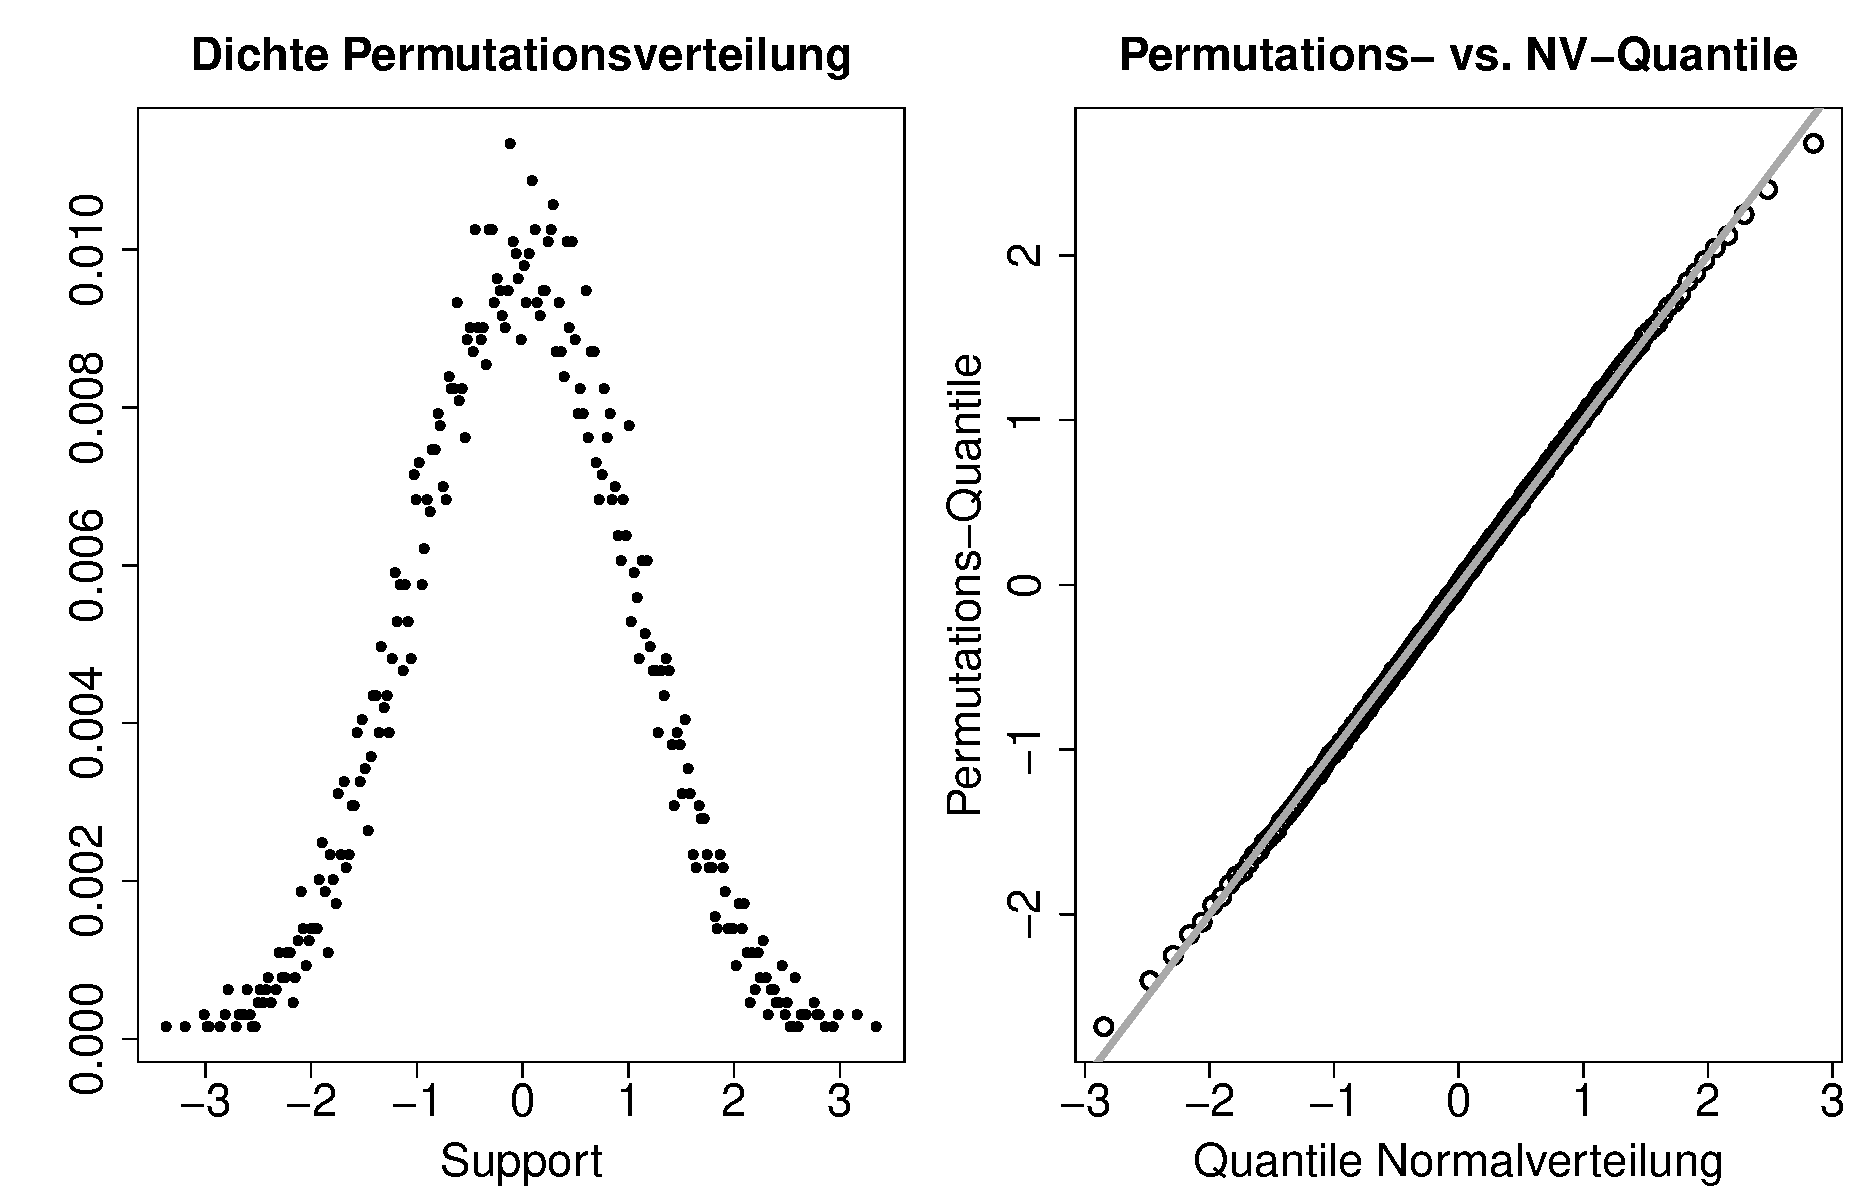
\includegraphics[width=12.5cm]{permDistrib}
\vspace*{-1em}
\caption{Dichteverteilung der Teststatistik des Permutationstests. Q-Q-Plot der Teststatistik des Permutationstests im Vergleich zur Standardnormalverteilung.}
\label{fig:permDistrib}
\end{figure}

Zum Vergleich mit dem Permutationstest soll zunächst der $p$-Wert des analogen parametrischen $t$-Tests ermittelt werden (Abschn.\ \ref{sec:tTwoInd}). Bei der folgenden manuellen Kontrolle dient die Mittelwertsdifferenz zwischen beiden Gruppen als Teststatistik. Dabei ist zu beachten, dass $\hat{\theta}^{\star}$ hier nicht für alle $N!$ möglichen Permutationen der Gesamtstichprobe vom Umfang $N$ bestimmt werden muss. Dies ist nur für jene Permutationen notwendig, die auch zu unterschiedlichen Gruppenzusammensetzungen führen, also nicht lediglich innerhalb jeder Gruppe die Reihenfolge vertauschen. Es gibt $N \choose n_{1}$ viele Möglichkeiten (Kombinationen, s.\ Abschn.\ \ref{sec:combinatorics}), zwei Gruppen der Größe $n_{1}$ und $n_{2}$ zu bilden, dabei ist jede Kombination gleich wahrscheinlich.
\begin{lstlisting}
# Vergleich: p-Wert aus analogem parametrischen t-Test
> tt <- t.test(values ~ ind, alt="less", var.equal=TRUE, data=dat)
> tt$p.value
[1] 0.01483469

# Indizes aller unterschiedlichen Zusammensetzungen Gruppe A*
> idx  <- seq_len(sum(Nj))            # Indizes Gesamt-Daten
> idxA <- combn(idx, Nj[1])           # alle n1-Kombinationen

# Mittelwertsdifferenz für gegebene Indizes x der Gruppe A*
> getDM <- function(x) {
+     mean(dat[x, "values"]) - mean(dat[-x, "values"])
+ }

> DMstar <- apply(idxA, 2, getDM)     # M-Differenz aller Kombinationen
> DMbase <- mean(DVa) - mean(DVb)     # beobachtete M-Differenz
\end{lstlisting}

Der für den $p$-Wert notwendige Vergleich $\hat{\theta}^{\star} \leq \hat{\theta}$ wird hier in zwei Vergleiche aufgeteilt, um robuster gegenüber Problemen der numerischen Repräsentation von Gleitkommazahlen zu sein (Abschn.\ \ref{sec:isTRUE}). Dafür wird nur auf ungefähre, nicht auf exakte Gleichheit von $\hat{\theta}^{\star}$ und $\hat{\theta}$ geprüft.
\begin{lstlisting}
# DMstar kleiner Basis-DM ODER DMstar ungefähr gleich Basis-DM?
> tol <- .Machine$double.eps^0.5      # numerische Toleranz
> DMsIsLEQ <- (DMstar < DMbase) | (abs(DMstar - DMbase) < tol)

# p-Wert: Anteil der mindestens so extremen Mittelwertsdifferenzen
> (pVal <- sum(DMsIsLEQ) / length(DMstar))
[1] 0.01756022
\end{lstlisting}

%Abbildung \ref{fig:permTest} zeigt den Vergleich des Histogramms der Mittelwertsdifferenzen mit der Dichtefunktion der unter $\text{H}_{0}$ gültigen Normalverteilung $\mathcal{N}(0, \sqrt{\frac{\sigma_{1}^{2}}{n_{1}} + \frac{\sigma_{2}^{2}}{n_{2}}})$ sowie den Vergleich der kumulierten relativen Häufigkeiten mit der entsprechenden Verteilungsfunktion.
%\begin{lstlisting}
%# Histogramm Mittelwertsdifferenzen aus Permutationstests
%> hist(resDM, freq=FALSE, breaks="FD", xlab="Mittelwertsdifferenzen",
%+      main="Permutationstest: Histogramm Mittelwertsdifferenzen")
%
%# füge Dichteverteilung passender Normalverteilung und Legende hinzu
%> curve(dnorm(x, 0, 20/sqrt(Nj[1]) + 20/sqrt(Nj[2])), lwd=2, add=TRUE)
%> legend(x="topright", lty=1, lwd=2, legend=expression(paste("N(0, ",
%+        sigma[1]^2 / n[1] + sigma[2]^2 / n[2], ")")))
%
%
%# kumulierte relative Häufigkeiten
%> plot(resDM, ecdf(resDM)(resDM), col="gray60", pch=16,
%>      xlab="Mittelwertsdifferenzen", ylab="kumulierte relative Häufigkeit",
%>      main="Kumulierte relative Häufigkeiten und Verteilungsfunktion")
%
%# füge Verteilungsfunktion passender Normalverteilung und Legende hinzu
%> curve(pnorm(x, 0, 20/sqrt(Nj[1]) + 20/sqrt(Nj[2])), lwd=2, add=TRUE)
%> legend(x="bottomright", lty=c(NA, 1), pch=c(16, NA), lwd=c(1, 2),
%>        col=c("gray60", "black"), legend=c("Permutationen",
%+        expression(paste("N(0, ", sigma[1]^2 / n[1] + sigma[2]^2 / n[2],
%+                         ")"))))
%\end{lstlisting}
%
%\begin{figure}[ht]
%\centering
%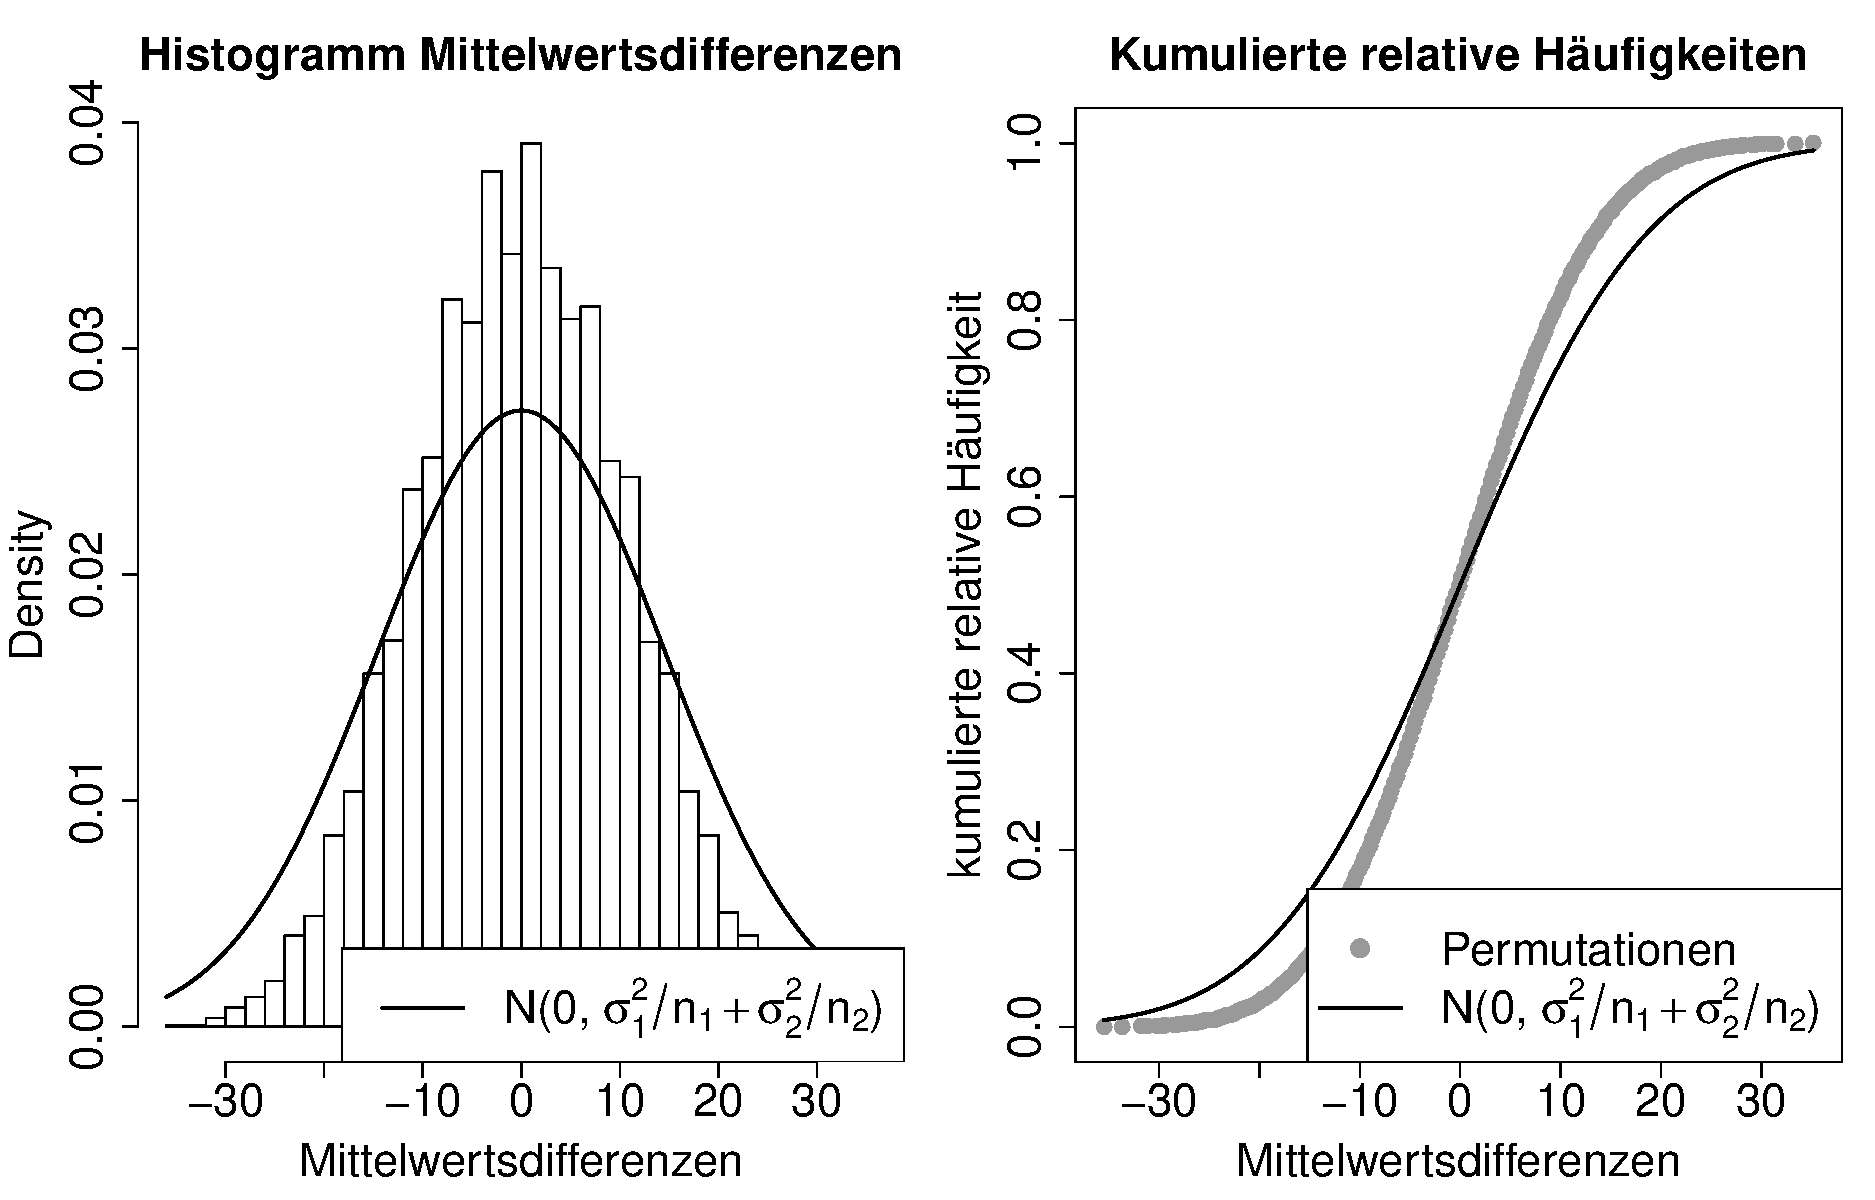
\includegraphics[width=12.5cm]{permTest}
%\vspace*{-1.5em}
%\caption{Histogramm der Mittelwertsdifferenzen aus einem Permutationstest mit Dichtefunktion der unter $\text{H}_{0}$ gültigen Normalverteilung. Kumulierte relative Häufigkeiten der Mittelwertsdifferenzen mit Verteilungsfunktion der Normalverteilung}
%\label{fig:permTest}
%\end{figure}

%%%%%%%%%%%%%%%%%%%%%%%%%%%%%%%%%%%%%%%%%%%%%%%%%%%%%%%%%%%%%%%%%%
%%%%%%%%%%%%%%%%%%%%%%%%%%%%%%%%%%%%%%%%%%%%%%%%%%%%%%%%%%%%%%%%%%
\subsection{Test auf gleiche Lageparameter in abhängigen Stichproben}
%%%%%%%%%%%%%%%%%%%%%%%%%%%%%%%%%%%%%%%%%%%%%%%%%%%%%%%%%%%%%%%%%%
%%%%%%%%%%%%%%%%%%%%%%%%%%%%%%%%%%%%%%%%%%%%%%%%%%%%%%%%%%%%%%%%%%

Beim Test auf Übereinstimmung von Verteilungen aus (hier zwei) abhängigen Stichproben hat die für \lstinline!oneway_test()! anzugebende Modellformel die Form \lstinline!<<AV>> ~ <<UV>> | <<BlockId>>!. Dabei codiert \lstinline!<<UV>>! als Faktor derselben Länge wie \lstinline!<<AV>>! den Messzeitpunkt. \lstinline!<<BlockId>>! ist ebenfalls ein solcher Faktor und gibt im Fall von Messwiederholung die Zugehörigkeit jedes Wertes zu einem Beobachtungsobjekt (bei gematchten Personen: zu einem Block) an.
\begin{lstlisting}
> N        <- 12                            # Anzahl Personen
> DVpre    <- round(rnorm(N, 100, 20))      # Daten Zeitpunkt prä
> DVpost   <- round(rnorm(N, 110, 20))      # Daten Zeitpunkt post
> datPP    <- stack(list(pre=DVpre, post=DVpost))   # Gesamt-Daten
> datPP$id <- factor(rep(1:N, times=2))     # Faktor Personen-ID

# Faktor Messzeitpunkt
> library(coin)                             # für oneway_test()
> oneway_test(values ~ ind | id, alternative="less",
+             distribution=approximate(B=9999), data=datPP)
Approximative 2-Sample Permutation Test
data: values by ind (pre, post) stratified by id
Z = -0.6056, p-value = 0.2748
alternative hypothesis: true mu is less than 0
\end{lstlisting}

Das Ergebnis des Fisher-Pitman Randomisierungstests soll zunächst mit dem $p$-Wert des analogen parametrischen $t$-Tests verglichen werden (Abschn.\ \ref{sec:tTwoDep}). Bei der anschließenden manuellen Kontrolle dient die mittlere paarweise Differenz zwischen den Werten der zwei abhängigen Bedingungen als Teststatistik. Dafür ist separat für jede Person die Zuordnung ihrer beiden Werte zu einem Testzeitpunkt zu permutieren. Dies ist äquivalent zur Permutation des Vorzeichens der personenweisen Messwertdifferenz. Bei $n$ Personen führt dies zu $2^{n}$ verschiedenen Gesamt-Permutationen.
\begin{lstlisting}
> tt <- t.test(values ~ ind, alt="less", paired=TRUE, data=datPP)
> tt$p.value
[1] 0.2839126

# alle 2^N Möglichk., pro Person Vorzeichen Differenz zu permutieren
> DVd    <- DVpre - DVpost          # personenweise Messwertdifferenzen
> ordLst <- lapply(numeric(N), function(x) { c(-1, 1) } )
> ordMat <- data.matrix(expand.grid(ordLst))   # alle 2^N Permutationen

# für Gesamt-Permutation x der Vorzeichen: mittlere personenweise Diff.
> getMD  <- function(x) { mean(abs(DVd) * x) }
> MDstar <- apply(ordMat, 1, getMD) # mittlere Differenzen alle Permut.
> MDbase <- mean(DVd)               # mittl. Differenz Basis-Stichprobe
\end{lstlisting}

Der für den $p$-Wert notwendige Vergleich $\hat{\theta}^{\star} \leq \hat{\theta}$ wird hier in zwei Vergleiche aufgeteilt, um robuster gegenüber Problemen der numerischen Repräsentation von Gleitkommazahlen zu sein (Abschn.\ \ref{sec:isTRUE}). Dafür wird nur auf ungefähre, nicht auf exakte Gleichheit von $\hat{\theta}^{\star}$ und $\hat{\theta}$ geprüft.
\begin{lstlisting}
# MDstar kleiner Basis-MD ODER MDstar ungefähr gleich Basis-MD?
> tol <- .Machine$double.eps^0.5     # numerische Toleranz
> MDsIsLEQ <- (MDstar < MDbase) | (abs(MDstar - MDbase) < tol)

# p-Wert: Anteil der mind. so extremen personenweisen Differenzen
> (pVal <- sum(MDsIsLEQ) / length(MDstar))
[1] 0.2800293
\end{lstlisting}

%%%%%%%%%%%%%%%%%%%%%%%%%%%%%%%%%%%%%%%%%%%%%%%%%%%%%%%%%%%%%%%%%%
%%%%%%%%%%%%%%%%%%%%%%%%%%%%%%%%%%%%%%%%%%%%%%%%%%%%%%%%%%%%%%%%%%
\subsection{Test auf Unabhängigkeit von zwei Variablen}
%%%%%%%%%%%%%%%%%%%%%%%%%%%%%%%%%%%%%%%%%%%%%%%%%%%%%%%%%%%%%%%%%%
%%%%%%%%%%%%%%%%%%%%%%%%%%%%%%%%%%%%%%%%%%%%%%%%%%%%%%%%%%%%%%%%%%

Für den Test auf Unabhängigkeit zweier an denselben Personen erhobener Variablen sollen hier dichotome Daten dienen, um das Ergebnis der manuellen Umsetzung mit jenem von Fishers exaktem Test vergleichen zu können -- dem passenden Permutationstest (Abschn.\ \ref{sec:fisherInd}).
\begin{lstlisting}
> Nf  <- 8                                    # Anzahl Personen
> DV1 <- rbinom(Nf, size=1, prob=0.5)         # Daten Zielgröße 1
> DV2 <- rbinom(Nf, size=1, prob=0.5)         # Daten Zielgröße 2

# p-Wert rechtsseitiger Test
> fisher.test(DV1, DV2, alternative="greater")$p.value
[1] 0.7857143
\end{lstlisting}

Die manuelle Kontrolle verwendet \lstinline!Permn(<<Vektor>>)!\index[func]{Permn()@\lstinline{Permn()}} aus dem Paket \lstinline!DescTools!\index[pack]{DescTools@\lstinline{DescTools}}, um die Zuordnung von Werten der zweiten AV zu jenen der ersten zu permutieren. Die Funktion erzeugt eine Matrix mit allen $n!$ vielen Permutationen des übergebenen Vektors in den Zeilen. Mit den Indizes für den Vektor der zweiten AV liefern diese Permutationen die gewünschten Zuordnungen und führen so zu allen möglichen Kontingenztafeln der gemeinsamen Häufigkeiten mit denselben Randhäufigkeiten wie in der Basisstichprobe. Teststatistik ist die Anzahl der in der Diagonale einer Kontingenztafel stehenden Fälle, also der Übereinstimmungen beider Variablen.
\begin{lstlisting}
# alle Nf! Zuordnungen AV1 <-> AV2: Matrix Permutationen Indizes 1:Nf
> library(DescTools)                          # für Permn()
> permIdx <- Permn(seq_len(Nf))

# Anzahl der Übereinstimmungen für gegebene Permutation x der AV 2
> getAgree <- function(x) { sum(diag(table(DV1, DV2[x]))) }

# Anzahl der Übereinstimmungen für jede der Nf! Permutationen
> resAgree <- apply(permIdx, 1, getAgree)
> agree12  <- sum(diag(table(DV1, DV2)))      # beobachtete Übereinst.

# p-Wert: Anteil der Permut. mit mindestens so großer Übereinstimmung
> (pVal <- sum(resAgree >= agree12) / length(resAgree))
[1] 0.7857143
\end{lstlisting}
